%=============================================================================%
% Author: 	John Joseph Valletta
% Date: 	09/04/2019
% Title: 	Fews slides on supervised learning
%=============================================================================%

% Preamble
 \documentclass[pdf]{beamer}
\usepackage[export]{adjustbox}
\usepackage{framed}
\usepackage{color}
\definecolor{dkgreen}{rgb}{0,0.6,0}
\definecolor{gray}{rgb}{0.5,0.5,0.5}
\definecolor{mauve}{rgb}{0.58,0,0.82}
\definecolor{deepblue}{rgb}{0,0,0.5}
\definecolor{deepred}{rgb}{0.6,0,0}
\definecolor{deepgreen}{rgb}{0,0.5,0}
\definecolor{lightgray}{rgb}{0.92,0.92,0.92}
\definecolor{myblue}{rgb}{0.12, 0.47, 0.71} 
\definecolor{tealblue}{rgb}{0, 0.5, 0.5}
\usepackage{listings} % to insert code
\usepackage{textpos} % textblock
\usepackage{verbatim}
\usepackage{hyperref}
\hypersetup{colorlinks=true, urlcolor=blue, linkcolor=black} 

% Presentation configuration
\mode<presentation>{\usetheme{Madrid}}
\usecolortheme[named=myblue]{structure}
\useinnertheme{circles} % circles, rectanges, rounded, inmargin
\usefonttheme[onlymath]{serif} % makes math fonts like the usual LaTeX ones
\setbeamercovered{transparent=4} % transparent
\setbeamertemplate{caption}{\raggedright\insertcaption\par} % Remove the word "Figure" from caption %\setbeamertemplate{caption}[default]
\setbeamertemplate{navigation symbols}{} % don't put navigation tools at the bottom (alternatively \beamertemplatenavigationsymbolsempty)
\graphicspath{ {./img/} }

% Titlepage
\title[Supervised Learning]{Supervised Learning}
%\subtitle{Built-in data types}
\author{John Joseph Valletta}
\date[April 2019]{April 2019}
\institute[]{University of Exeter, Penryn Campus, UK}
\titlegraphic{
\hfill

\includegraphics[width=\textwidth, keepaspectratio]{logo.jpg}}

%=============================================================================%
%=============================================================================%
% Start of Document
%=============================================================================%
%=============================================================================%
\begin{document}

%=============================================================================%
%=============================================================================%
\begin{frame}
\titlepage
\end{frame}

%=============================================================================%
%=============================================================================%
\begin{frame}{Overview}
\begin{itemize}\addtolength{\itemsep}{0.5\baselineskip}
	\item What is supervised learning?
	\item Cross-validation
	\item $k$-nearest neighbour ($kNN$)
	\item Decision trees
	\item Random forests
	\item Support vector machines
\end{itemize}
\end{frame}

%=============================================================================%
%=============================================================================%
\begin{frame}{What's the problem?}
\begin{center}
\begin{figure}
	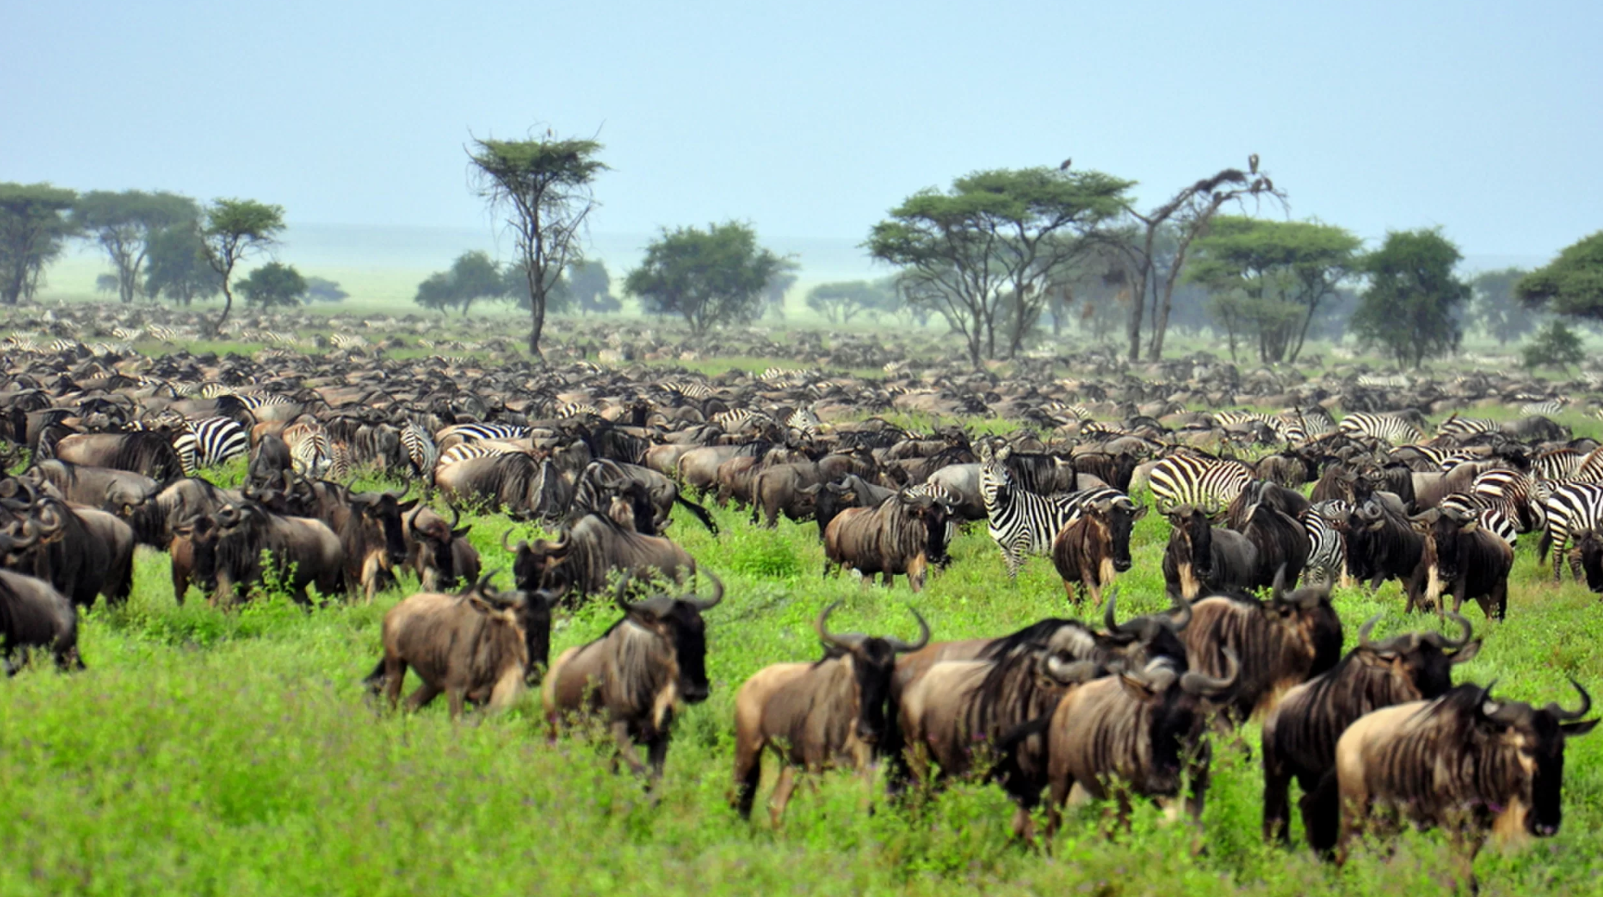
\includegraphics[width=0.9\textwidth]{04-serengeti.png}
\end{figure}
\end{center}
\vfill
\centering
\visible<2->{{\small https://www.livescience.com/23310-serengeti.html}}
\end{frame}

%=============================================================================%
%=============================================================================%
\begin{frame}{Counting wildebeest}
\centering
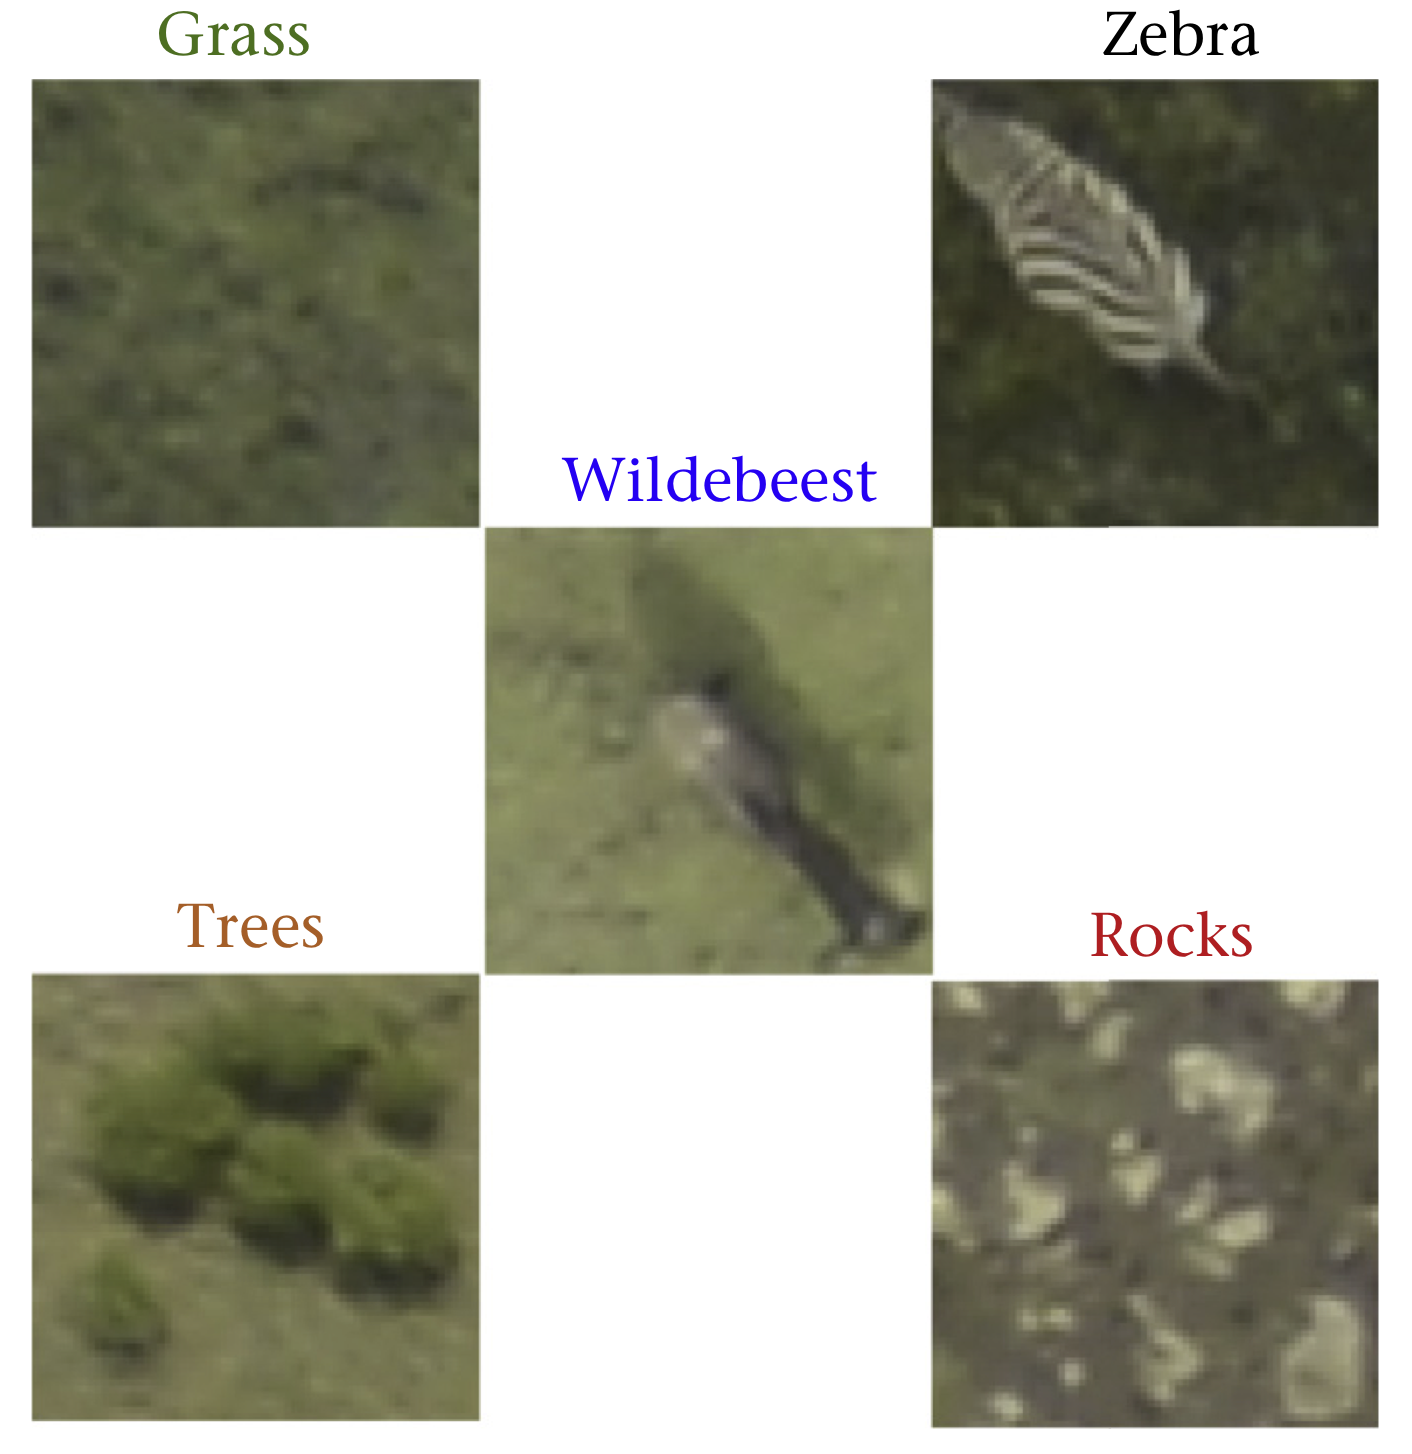
\includegraphics[width=0.48\textwidth]{04-UAV.png}\hfill
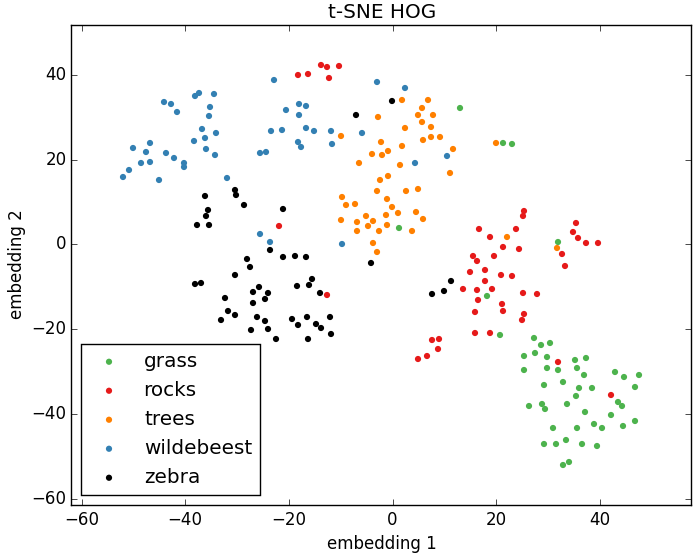
\includegraphics[width=0.48\textwidth]{tsne_hog.png}
\end{frame}

%=============================================================================%
%=============================================================================%
\begin{frame}{What is supervised learning?}
\begin{block}{}
Supervised learning methods determine the mapping (\textbf{predictive model}) between a set of features 
and a continuous outcome (\textbf{regression}), or a categorical variable (\textbf{classification})
\end{block}
\vfill
\centering
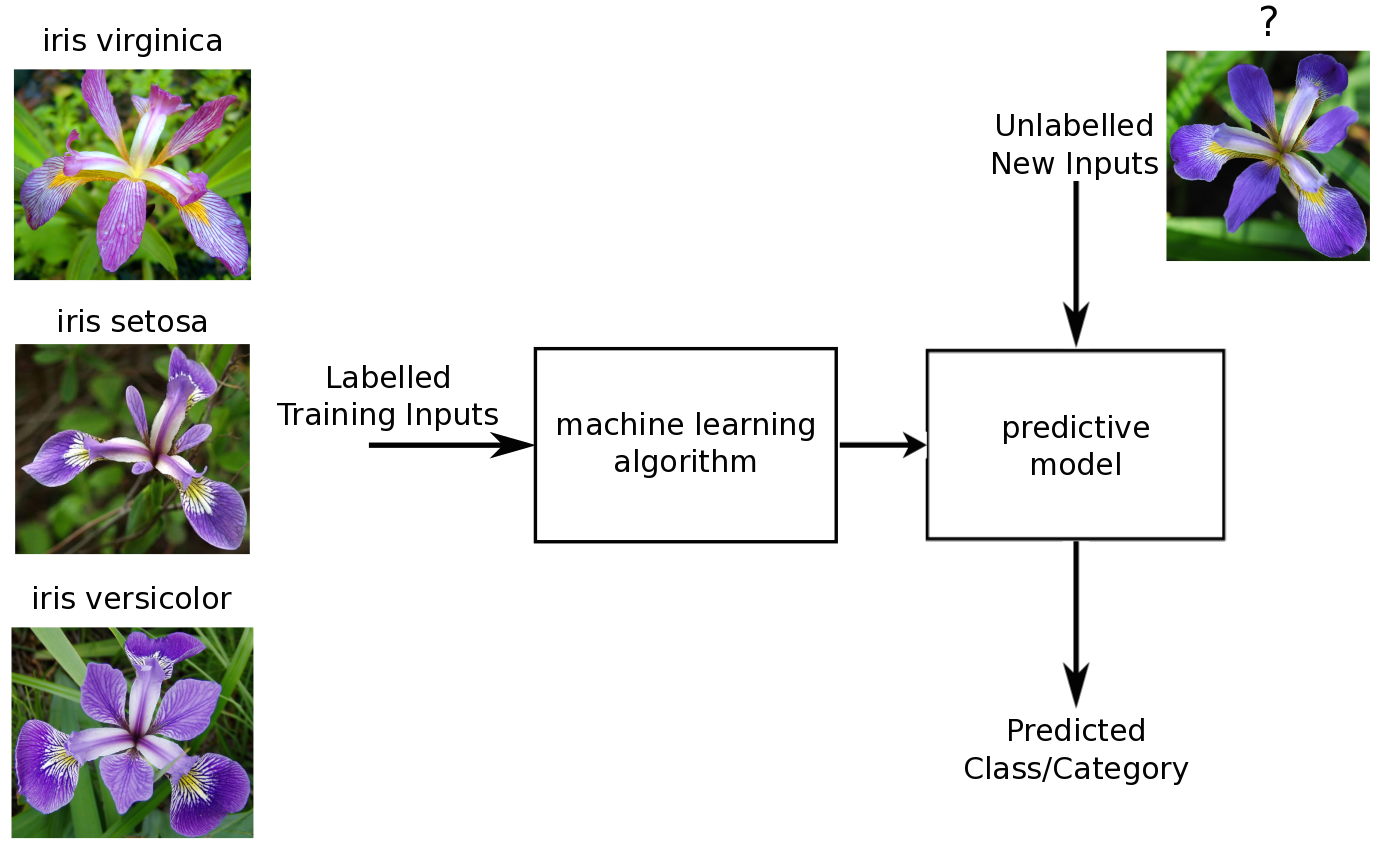
\includegraphics[width=0.7\textwidth]{classification.png}
\end{frame}

%=============================================================================%
%=============================================================================%
\begin{frame}{Bias-variance tradeoff}
\begin{itemize}\addtolength{\itemsep}{0.5\baselineskip}
	\item Machine learning algorithms are very flexible in order to deal with complex data
	\item So how \textit{well} should we fit to the training data to get good generalisation?
	\item Driving the training error to zero is \textit{not} a good idea
\end{itemize}
\vfill
\begin{center}
\visible<2->{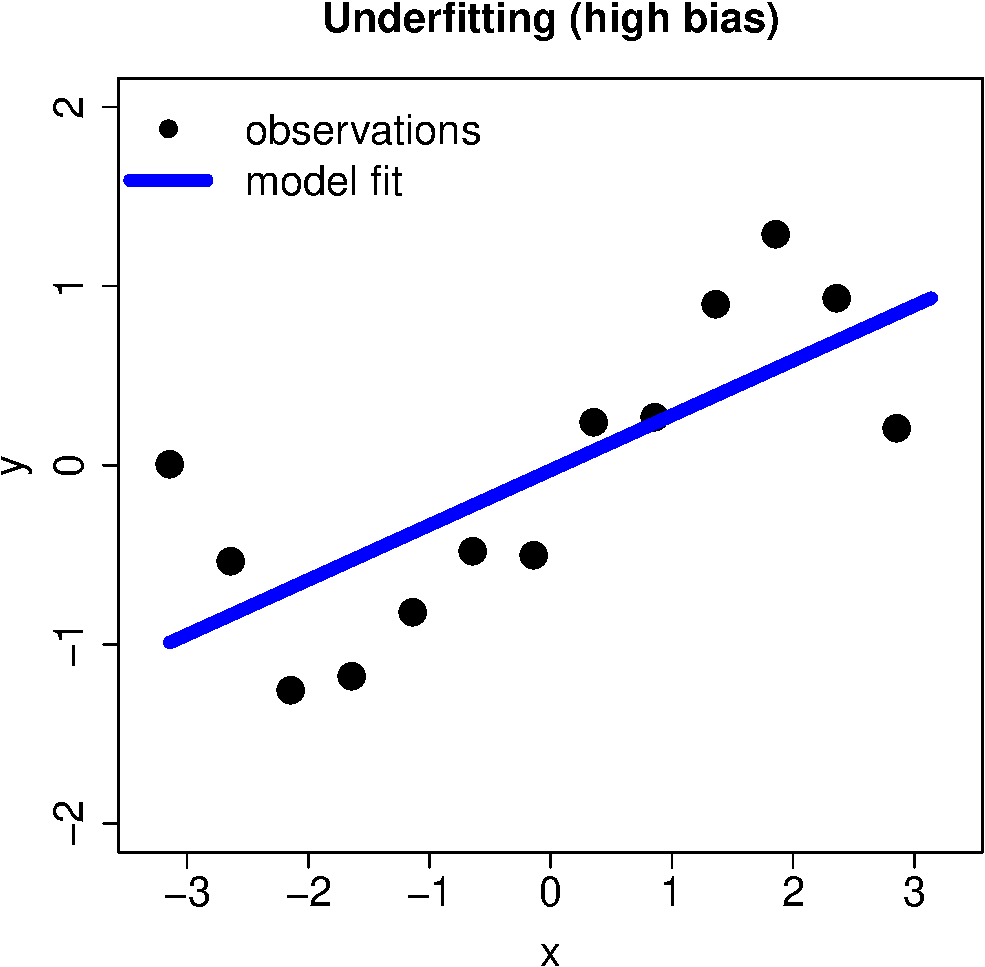
\includegraphics[width=0.3\textwidth]{polyFit1.pdf}}
\visible<3->{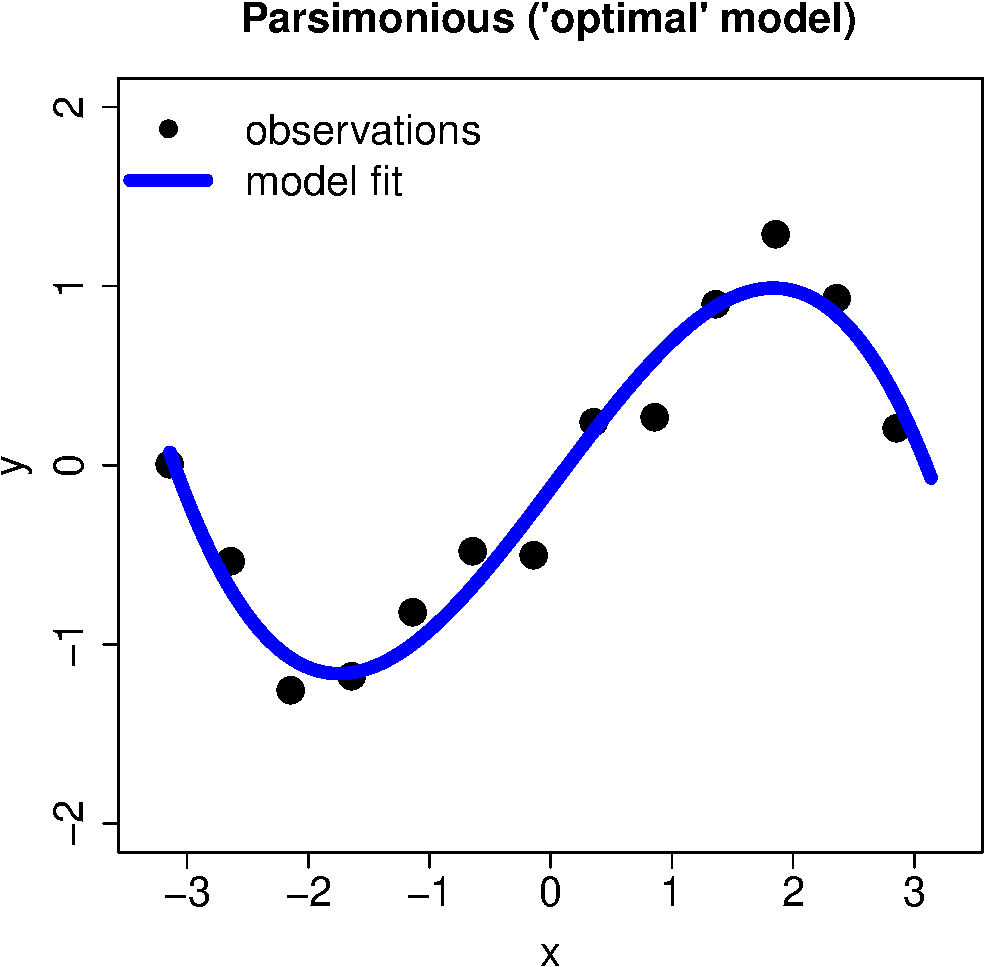
\includegraphics[width=0.3\textwidth]{polyFit3.pdf}}
\visible<4->{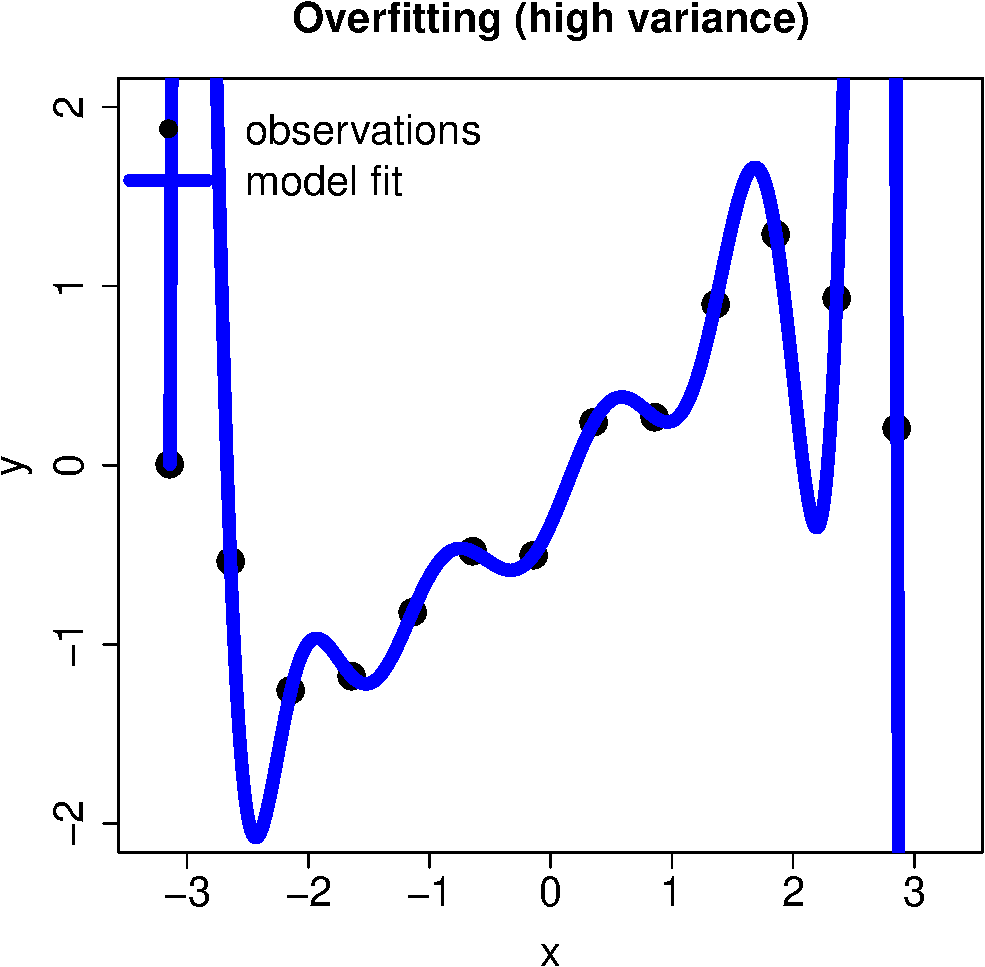
\includegraphics[width=0.3\textwidth]{polyFit12.pdf}}
\end{center}
\end{frame}

%=============================================================================%
%=============================================================================%
\begin{frame}{Cross-validation}

\begin{itemize}\addtolength{\itemsep}{0.25\baselineskip}
	\item The flexibility of ML models is constrained by \textbf{tuning} their \textbf{hyperparameters}
	\item \textbf{$k$-fold cross-validation} allow us to find optimal hyperparameters
\end{itemize}

\begin{center}
\vfill
\centering
\visible<2->{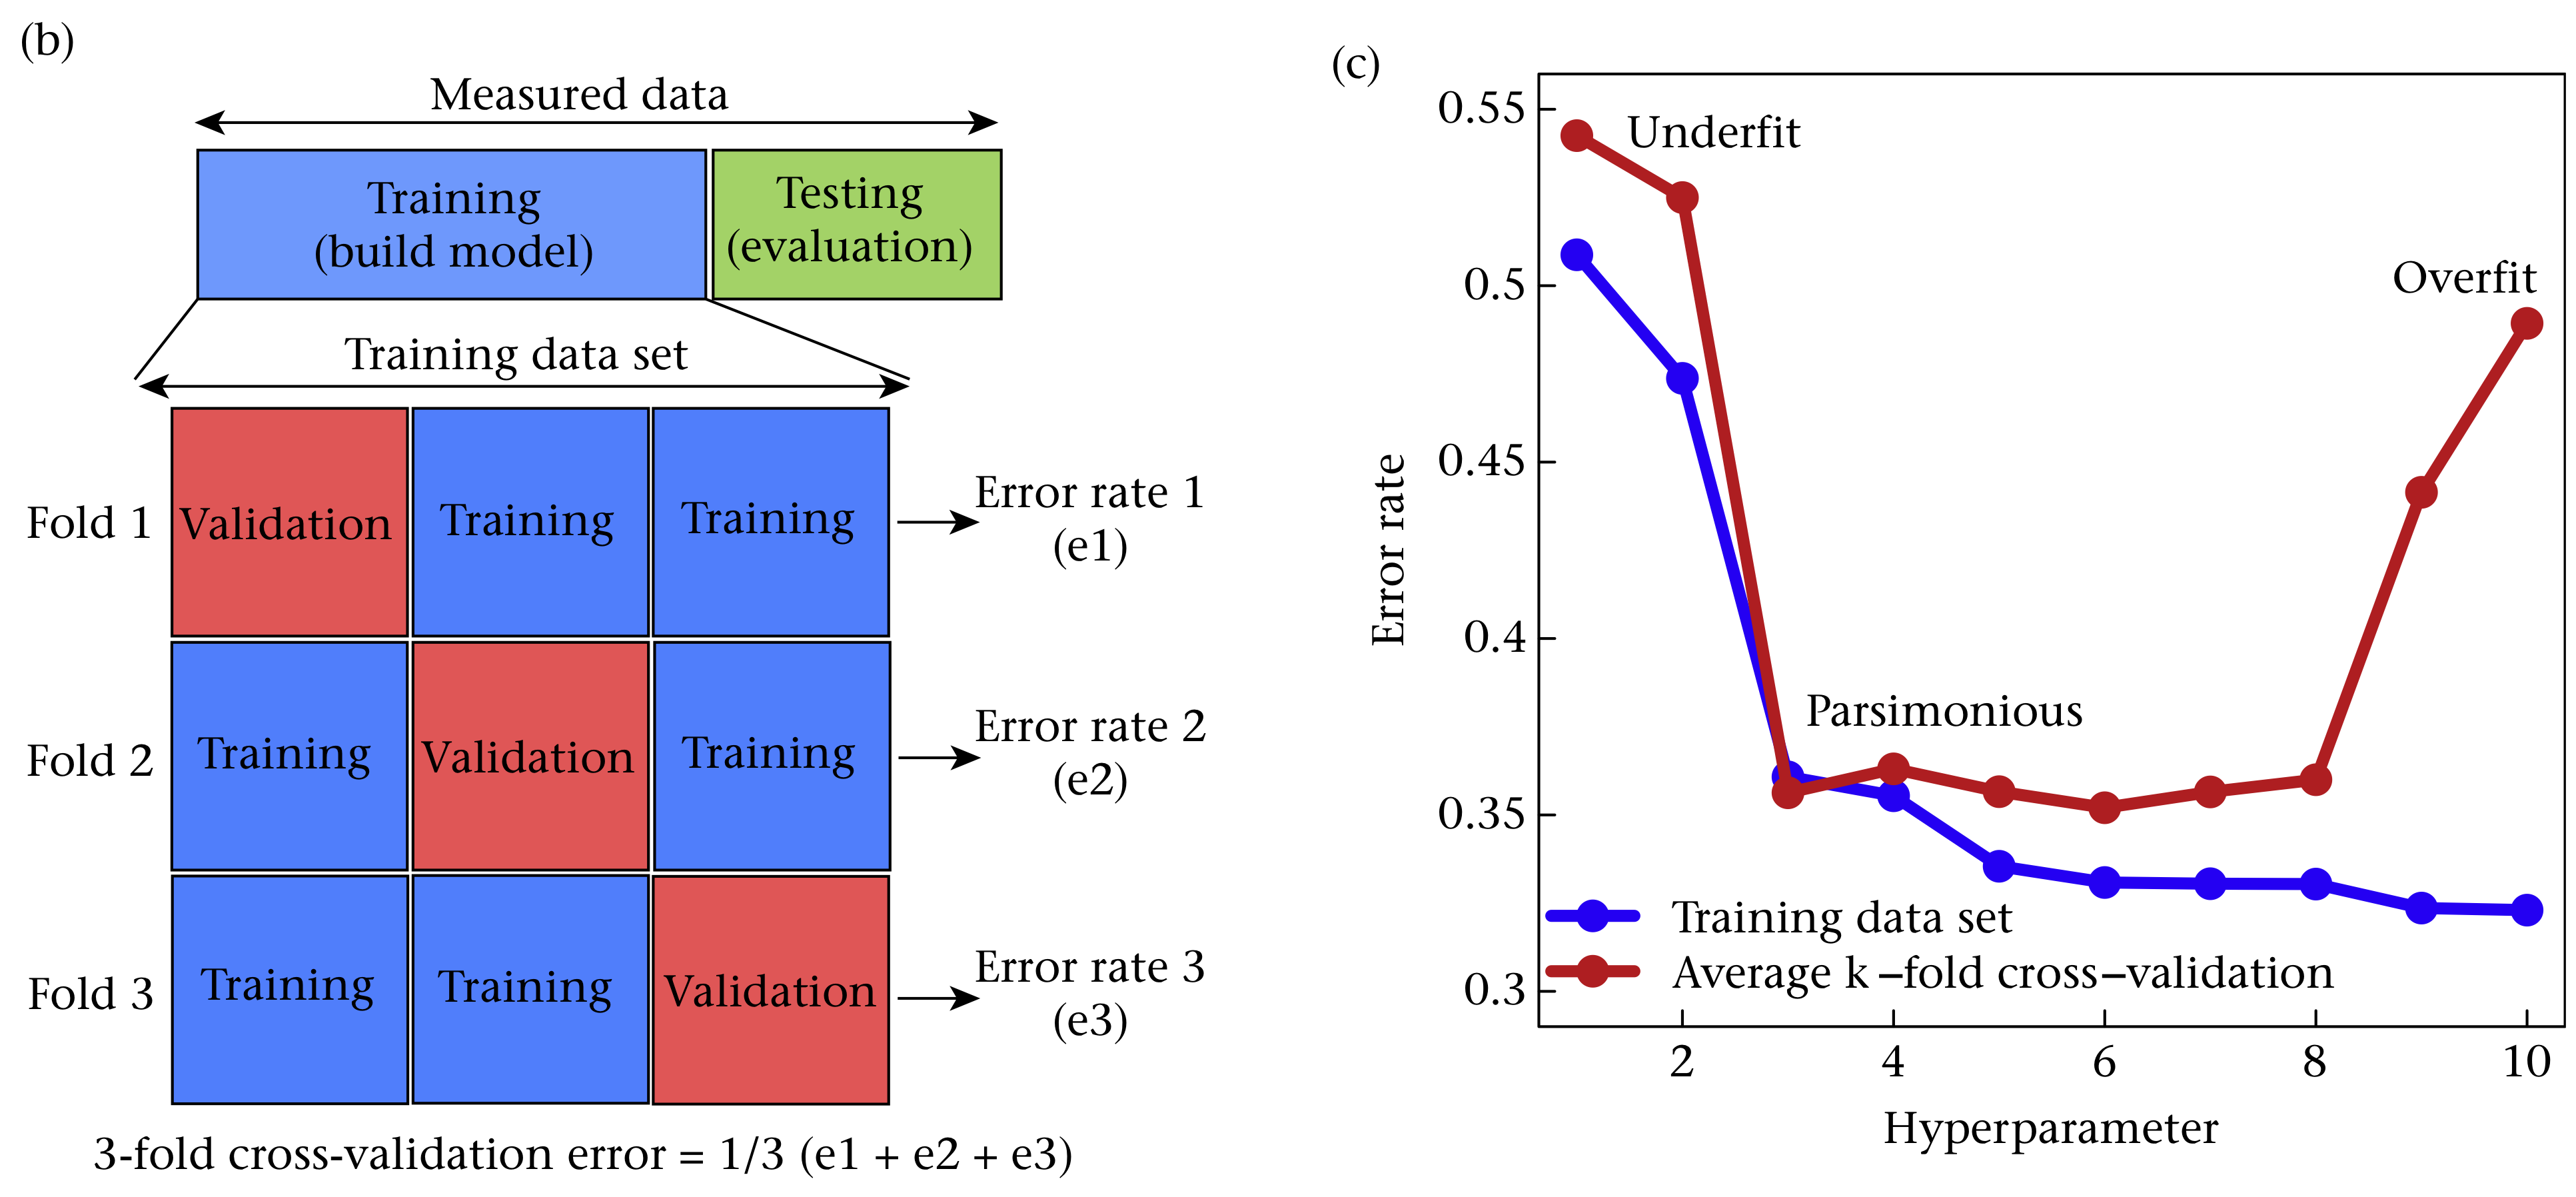
\includegraphics[width=0.85\textwidth]{crossvalidation.png}}
\end{center}
\end{frame}

%=============================================================================%
%=============================================================================%
\begin{frame}{Predictive performance measures}

\begin{itemize}\addtolength{\itemsep}{.75\baselineskip}
	\item To compare models during cross-validation \textbf{predictive performance measures} are computed
	\item Several metrics exist, some of the more popular ones are:
	\begin{itemize}
		\item \textbf{Regression}: root mean squared error (RMSE), R-squared
		\item \textbf{Classification}: area uder the ROC curve, confusion matrix
	\end{itemize}
\end{itemize}
\vfill
\centering
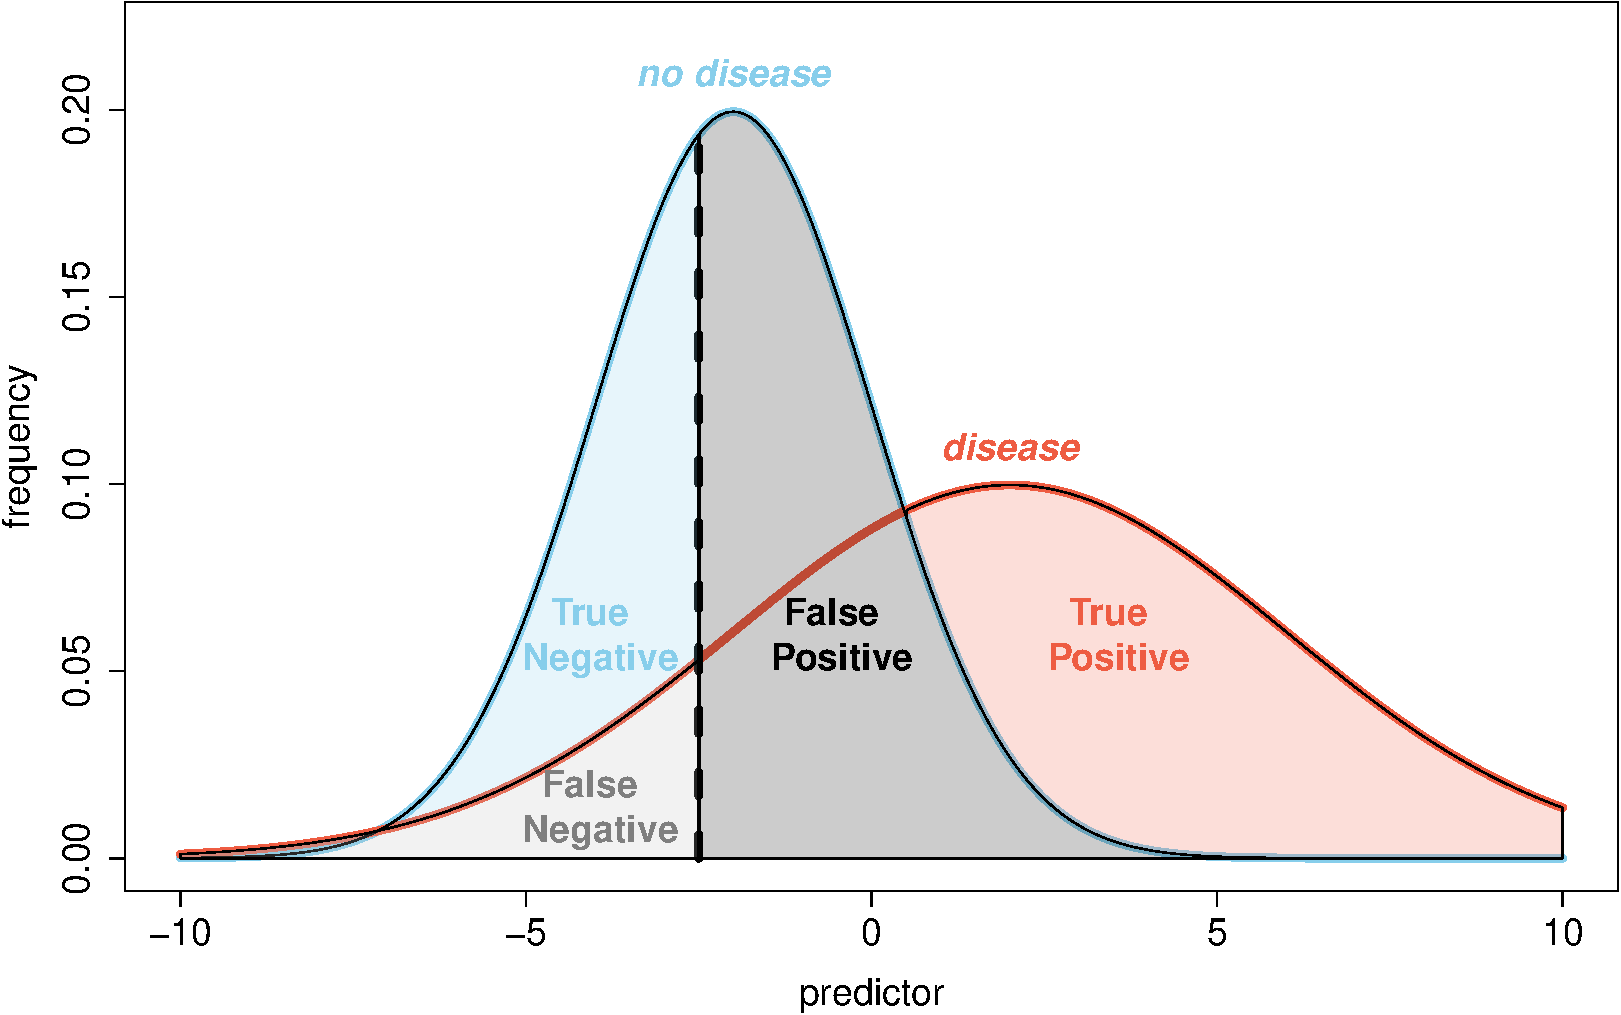
\includegraphics[width=0.45\textwidth]{binaryclassifier.pdf}\hspace{1cm}
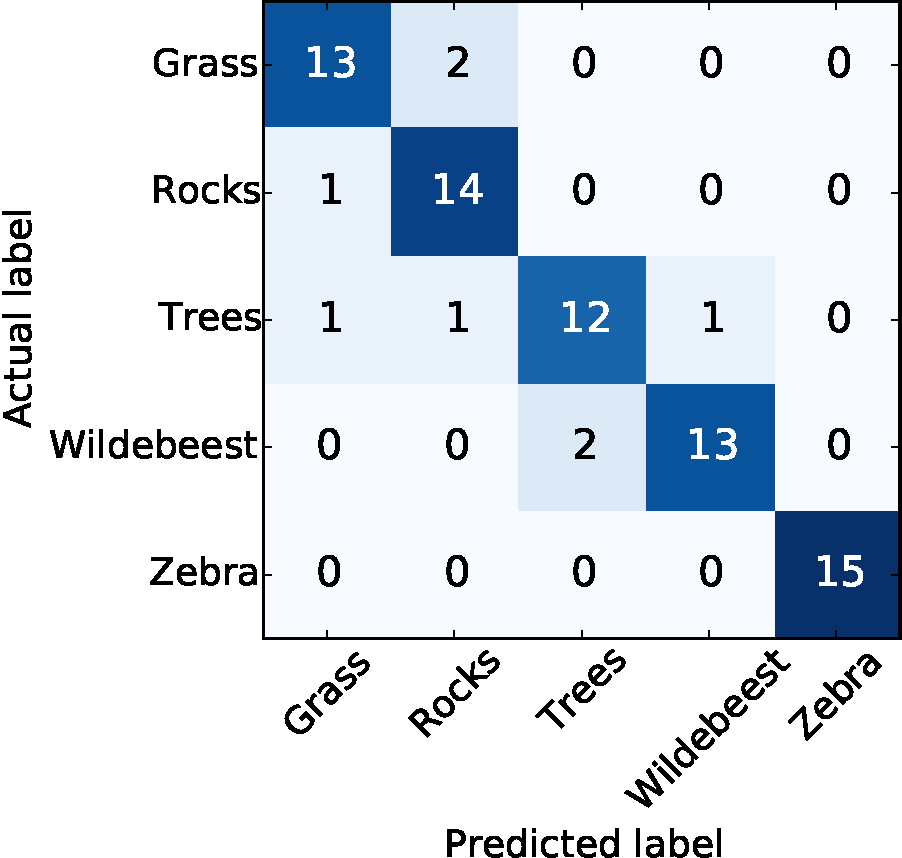
\includegraphics[width=0.3\textwidth]{confusionmatrix.pdf}

\end{frame}

%=============================================================================%
%=============================================================================%
\begin{frame}{$k$-nearest neighbour ($k$NN)}
\begin{enumerate}\addtolength{\itemsep}{2\baselineskip}
	\item<2-> Calculate distance between test point and every training data point 
	\item<3-> Find the $k$ training points closest to test point 
	\item<4-> Assign test point the majority vote of their class label
\end{enumerate}
\end{frame}

%=============================================================================%
%=============================================================================%
\begin{frame}{$k$-nearest neighbour}
	\begin{center}
		\includegraphics<1>[width=0.65\textwidth]{kNN01.pdf}
		\includegraphics<2>[width=0.65\textwidth]{kNN05.pdf}
		\includegraphics<3>[width=0.65\textwidth]{kNN15.pdf}
		\includegraphics<4>[width=0.65\textwidth]{kNN30.pdf}
	\end{center}
\end{frame}

%=============================================================================%
%=============================================================================%
\begin{frame}{$k$-nearest neighbour}
\begin{exampleblock}{Pros}
\begin{itemize}
	\item Simple and intuitive
	\item Works for multi-class problems
	\item Non-linear decision boundaries 
	\item $k$ easily tuned by cross-validation  
\end{itemize}
\end{exampleblock}
\vfill
\begin{alertblock}{Cons}
\begin{itemize}
	\item Can be computationally expensive, as for every test point, distance to \textit{every} training data point needs to be computed
	\item Takes up a lot of storage as \textit{all} training points need to be retained
\end{itemize}
\end{alertblock}
\end{frame}

%=============================================================================%
%=============================================================================%
\begin{frame}{Decision trees}
\begin{enumerate}\addtolength{\itemsep}{2\baselineskip}
	\item<2-> Find the yes/no rule that best splits the data with respect to \textit{one} of the features
	\item<3-> The best split is the one that produces the most homogeneous groups; found by maximising information gain/lowering entropy.
	\item<4-> Repeat steps 1 to 2 until all data are correctly classified or some stopping rule reached.
\end{enumerate}
\end{frame}

%=============================================================================%
%=============================================================================%
\begin{frame}{Decision trees}
\begin{center}
	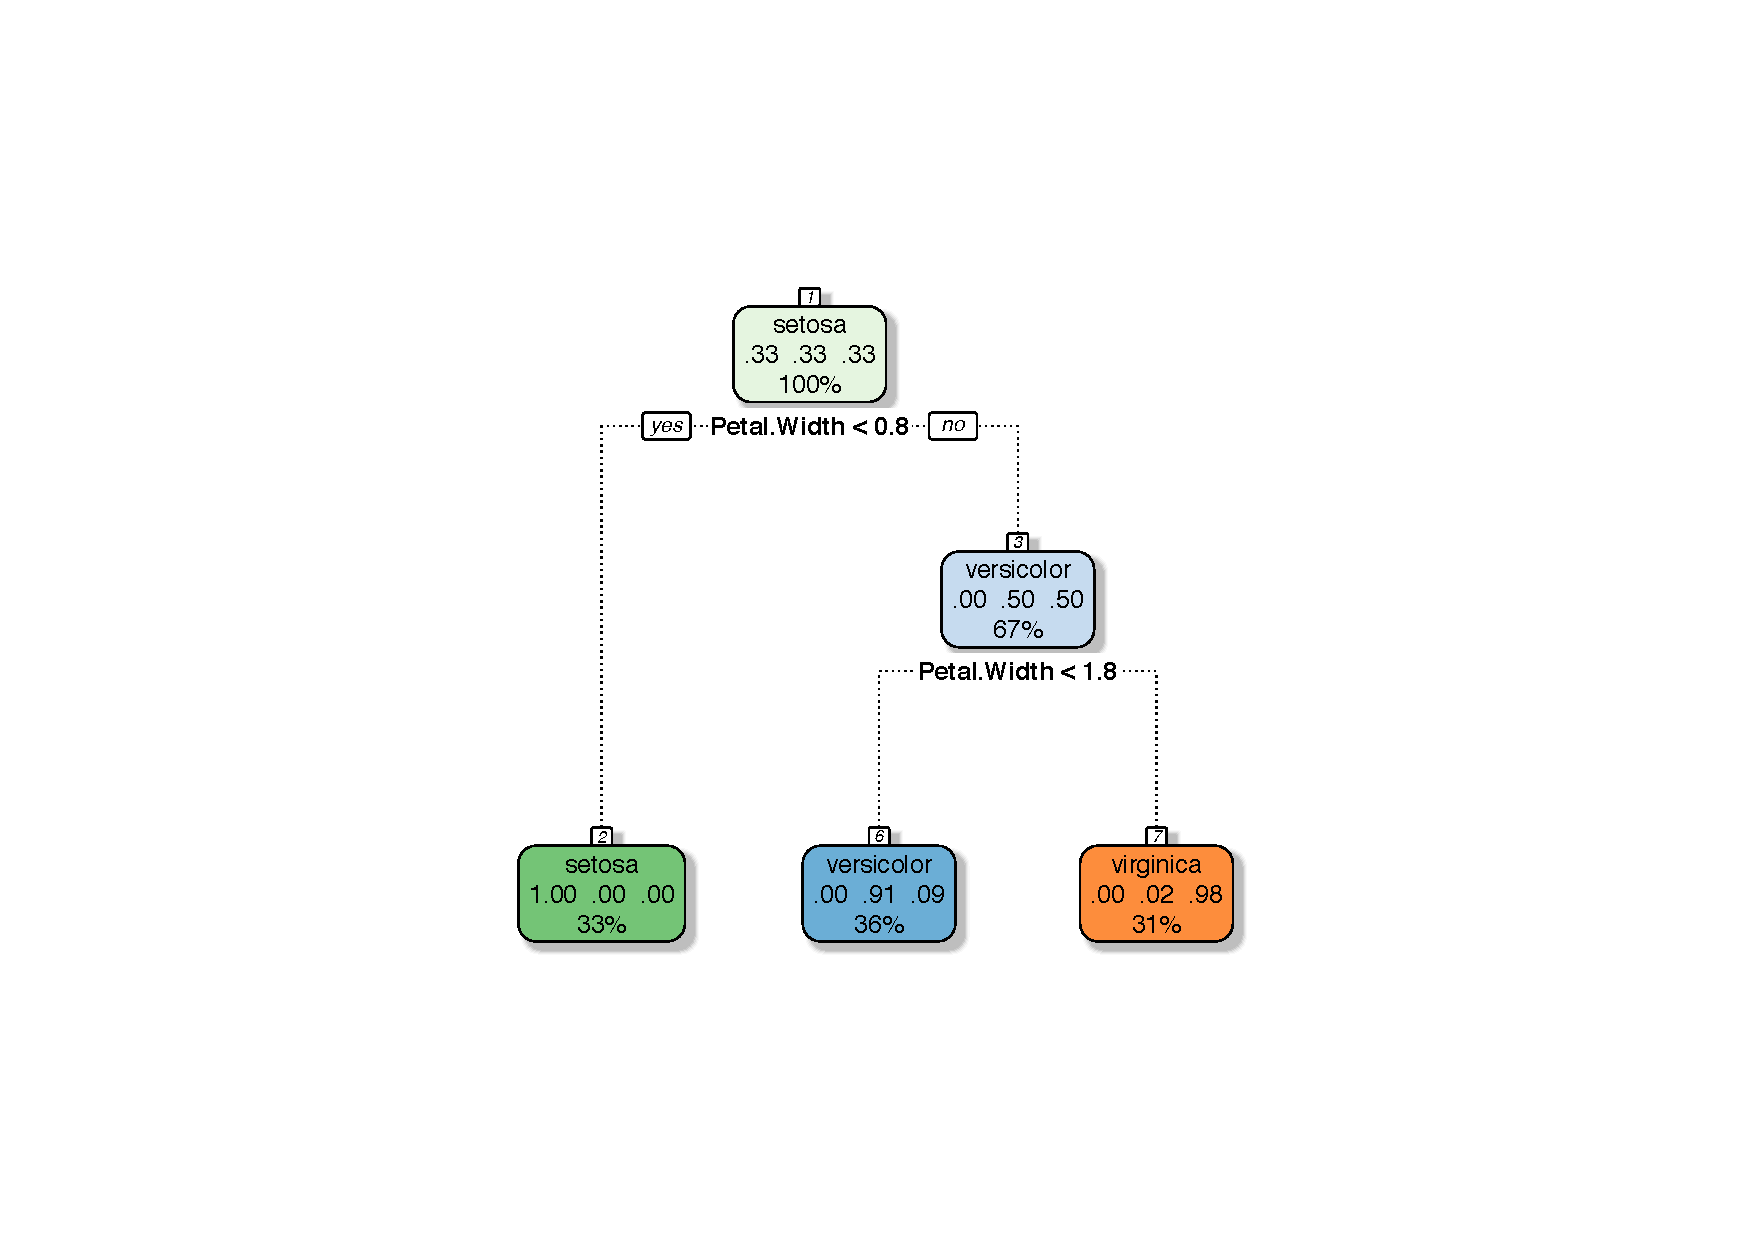
\includegraphics[width=0.7\textwidth]{niceTree.pdf}	
\end{center}
\end{frame}

%=============================================================================%
%=============================================================================%
\begin{frame}{Decision boundaries}
\begin{center}
	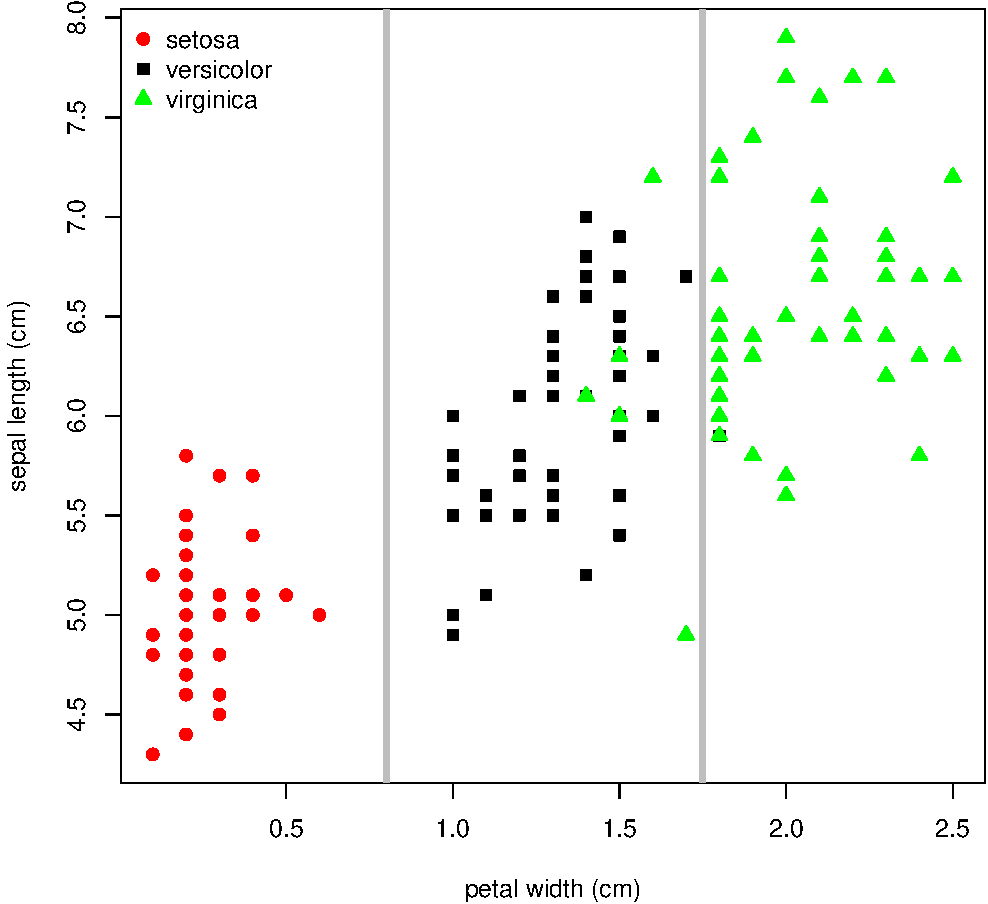
\includegraphics[width=0.7\textwidth]{irisPlotBound.pdf}
\end{center}
\end{frame}

%=============================================================================%
%=============================================================================%
\begin{frame}{Decision trees}
\begin{exampleblock}{Pros}
\begin{itemize}
	\item Model is very easy to explain to non-experts and can be directly used to generate rules
	\item Computationaly inexpensive to train, evaluate and store 
	\item Handle both categorical and continuous data 
	\item Robust to outliers
\end{itemize}
\end{exampleblock}
\vfill
\begin{alertblock}{Cons}
\begin{itemize}
	\item Can easily overfit the data
	\item Predictive accuracy can be poor
	\item Linear decision boundaries 
	\item Small changes to training data may lead to a completely different tree
\end{itemize}
\end{alertblock}
\end{frame}

%=============================================================================%
%=============================================================================%
\begin{frame}{Random forests}
\begin{itemize}\addtolength{\itemsep}{0.1\baselineskip}
	\item<2-> Decision trees are intuitive but suffer from overfitting which significantly affect their predictive accuracy
	\item<3-> \textbf{Pruning}, to ``trim'' the tree back, help reduce this overfit
	\item<4-> \textbf{Ensemble} methods such as Random Forests are a better alternative
	\item<5-> \textbf{Rationale}: Instead of one tree, grow a \textit{forest}, where every bushy tree (no pruning) is a bit different,
	then average predictions over all trees
\end{itemize}
\vfill
\visible<5->{
\begin{center}
	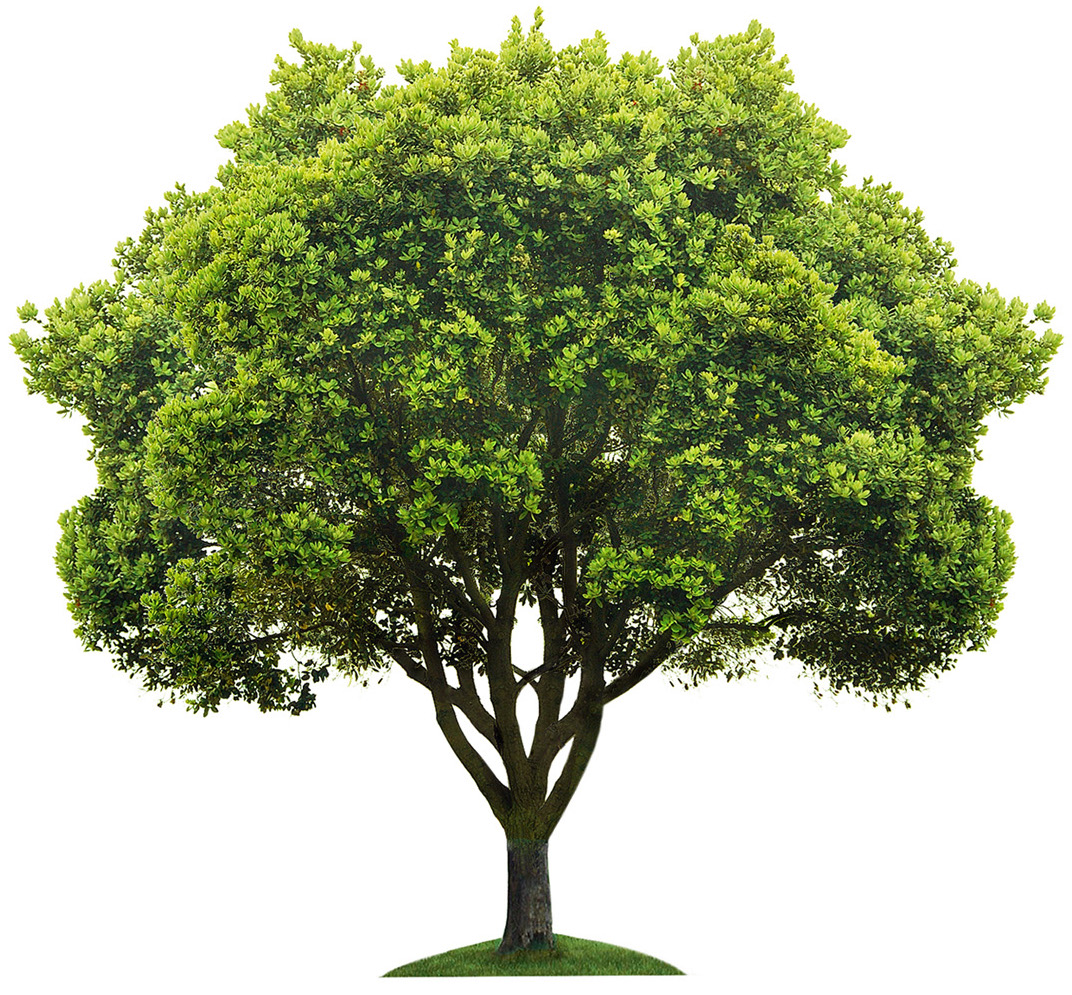
\includegraphics[width=0.32\textwidth]{tree.jpg}
	\Huge $\Rightarrow$ \normalsize
	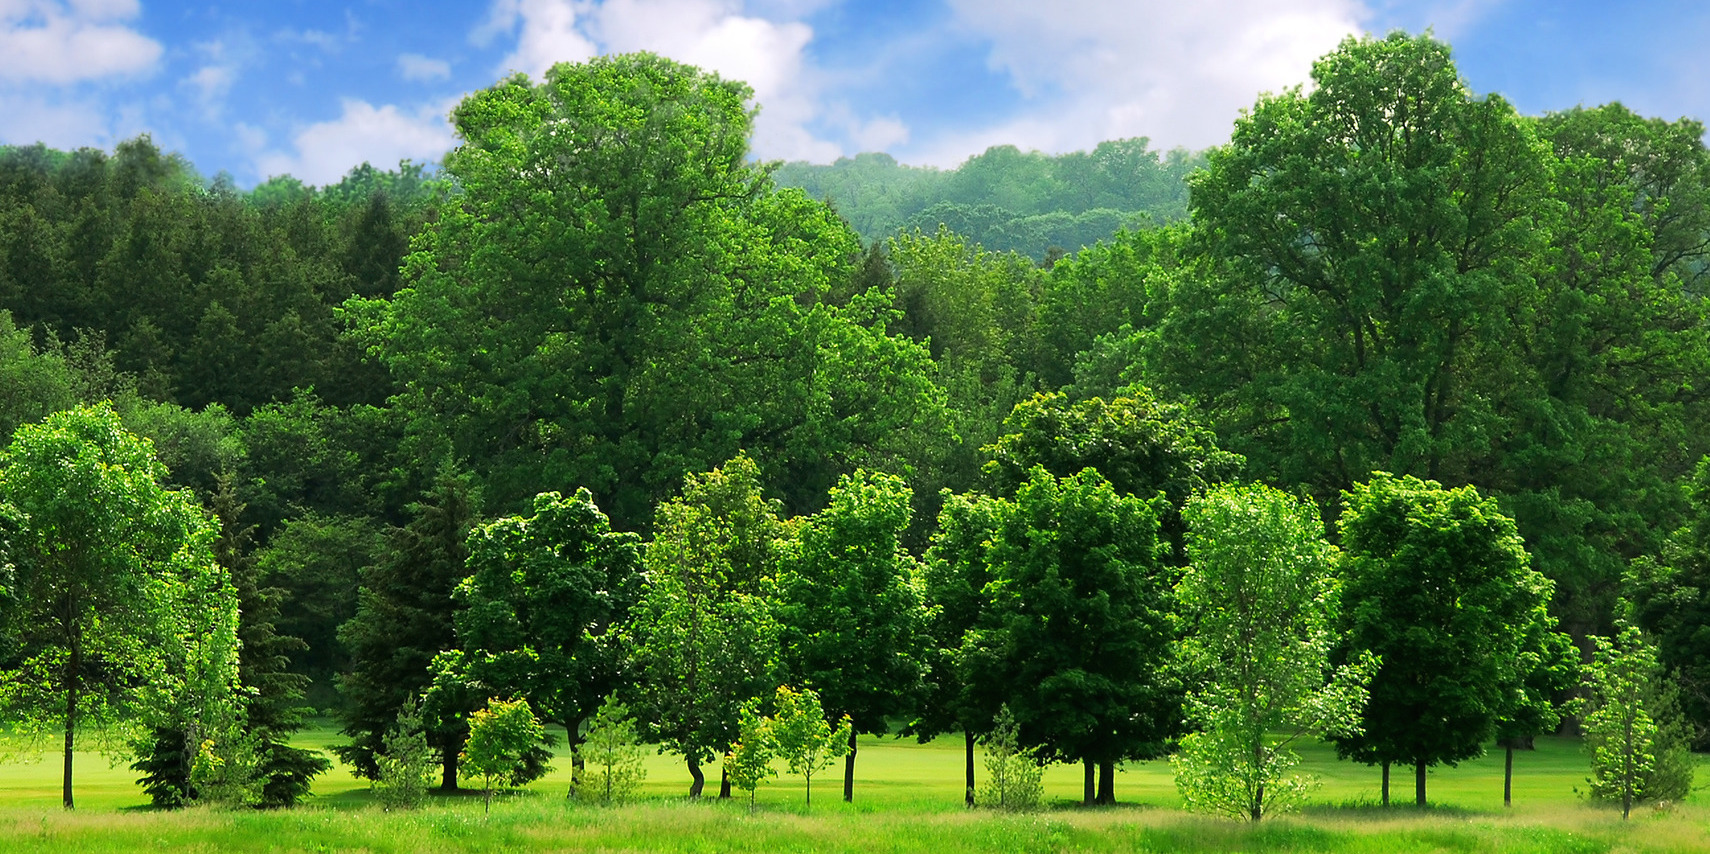
\includegraphics[width=0.58\textwidth]{forest.jpg}
\end{center}}
\end{frame}

%=============================================================================%
%=============================================================================%
\begin{frame}{Random forests}
\begin{enumerate}\addtolength{\itemsep}{2\baselineskip}
	\item<2-> Grow $T$ decorrelated trees (no pruning)
	\item<3-> Forest randomness is induced by:
		\begin{itemize}
			\item<3-> Bagging (\textbf{B}ootstrap \textbf{AGG}regat\textbf{ING}), each tree is trained
			on a subset of the data randomly sampled with replacement
			\item<3-> Considering only a subset of predictors as candidates for each split
		\end{itemize}
	\item<4-> Average predictions from all $T$ trees.
\end{enumerate}
\end{frame}

%=============================================================================%
%=============================================================================%
\begin{frame}{De-correlated trees}
	\begin{center}
		\includegraphics<1>[width=0.68\textwidth]{treeFit1.pdf}
		\includegraphics<2>[width=0.6\textwidth]{treeFit2.pdf}
	\end{center}
\end{frame}

%=============================================================================%
%=============================================================================%
\begin{frame}{Variable importance}
\begin{itemize}\addtolength{\itemsep}{2\baselineskip}
	\item Cannot visualise decision boundaries (loss of interpretability)
	\item However, variable importance helps us perform feature selection 
\end{itemize}

\begin{center}
	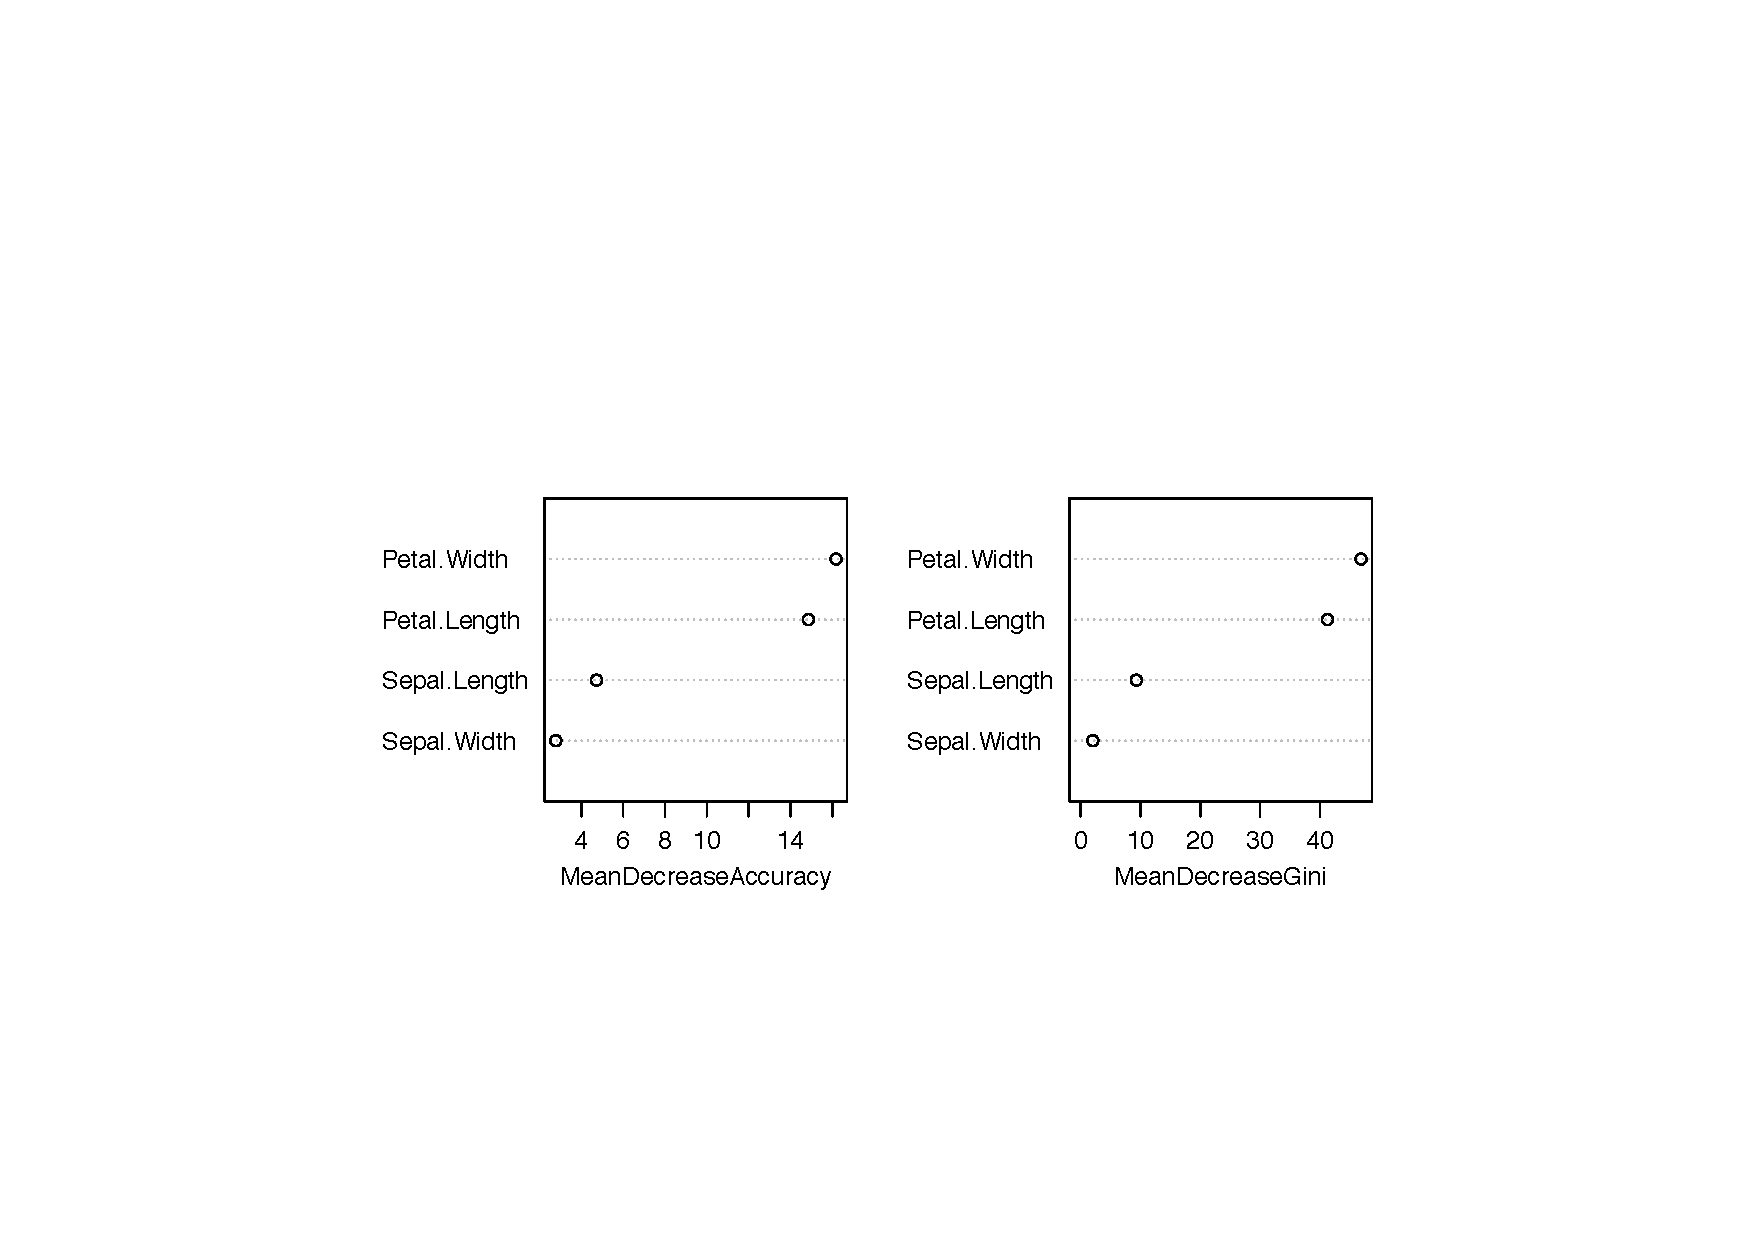
\includegraphics[width=0.85\textwidth]{varImportance.pdf}
\end{center}
\end{frame}


%=============================================================================%
%=============================================================================%
\begin{frame}{Random forests}
\begin{exampleblock}{Pros}
\begin{itemize}
	\item State-of-the-art predictive accuracy
	\item Can handle thousands of both categorical and continuous predictors without variable deletion
	\item Robust to outliers
	\item Estimates the importance of every predictor
	\item Out-of-bag error (unbiased estimate of test error for every tree built)
	\item Can cope with unbalanced datasets by setting class weights
	\item Trivially parallelisable
\end{itemize}
\end{exampleblock}
\vfill
\begin{alertblock}{Cons}
\begin{itemize}
	\item Harder to interpret then plain decision trees
\end{itemize}
\end{alertblock}
\end{frame}

%=============================================================================%
%=============================================================================%
\begin{frame}{Support vector machines (SVMs)}
Which is the best separating line?
	\begin{center}
		\includegraphics<1>[width=0.65\textwidth]{svmSepLine1.pdf}
		\includegraphics<2>[width=0.65\textwidth]{svmSepLine2.pdf}
		\includegraphics<3>[width=0.65\textwidth]{svmSepLine3.pdf}
		\includegraphics<4>[width=0.65\textwidth]{svmSepLine4.pdf}
	\end{center}
\end{frame}

%=============================================================================%
%=============================================================================%
\begin{frame}{Maximal margin classifier}
\textbf{Rationale}: Maximise the \textit{margin}
\begin{center}
		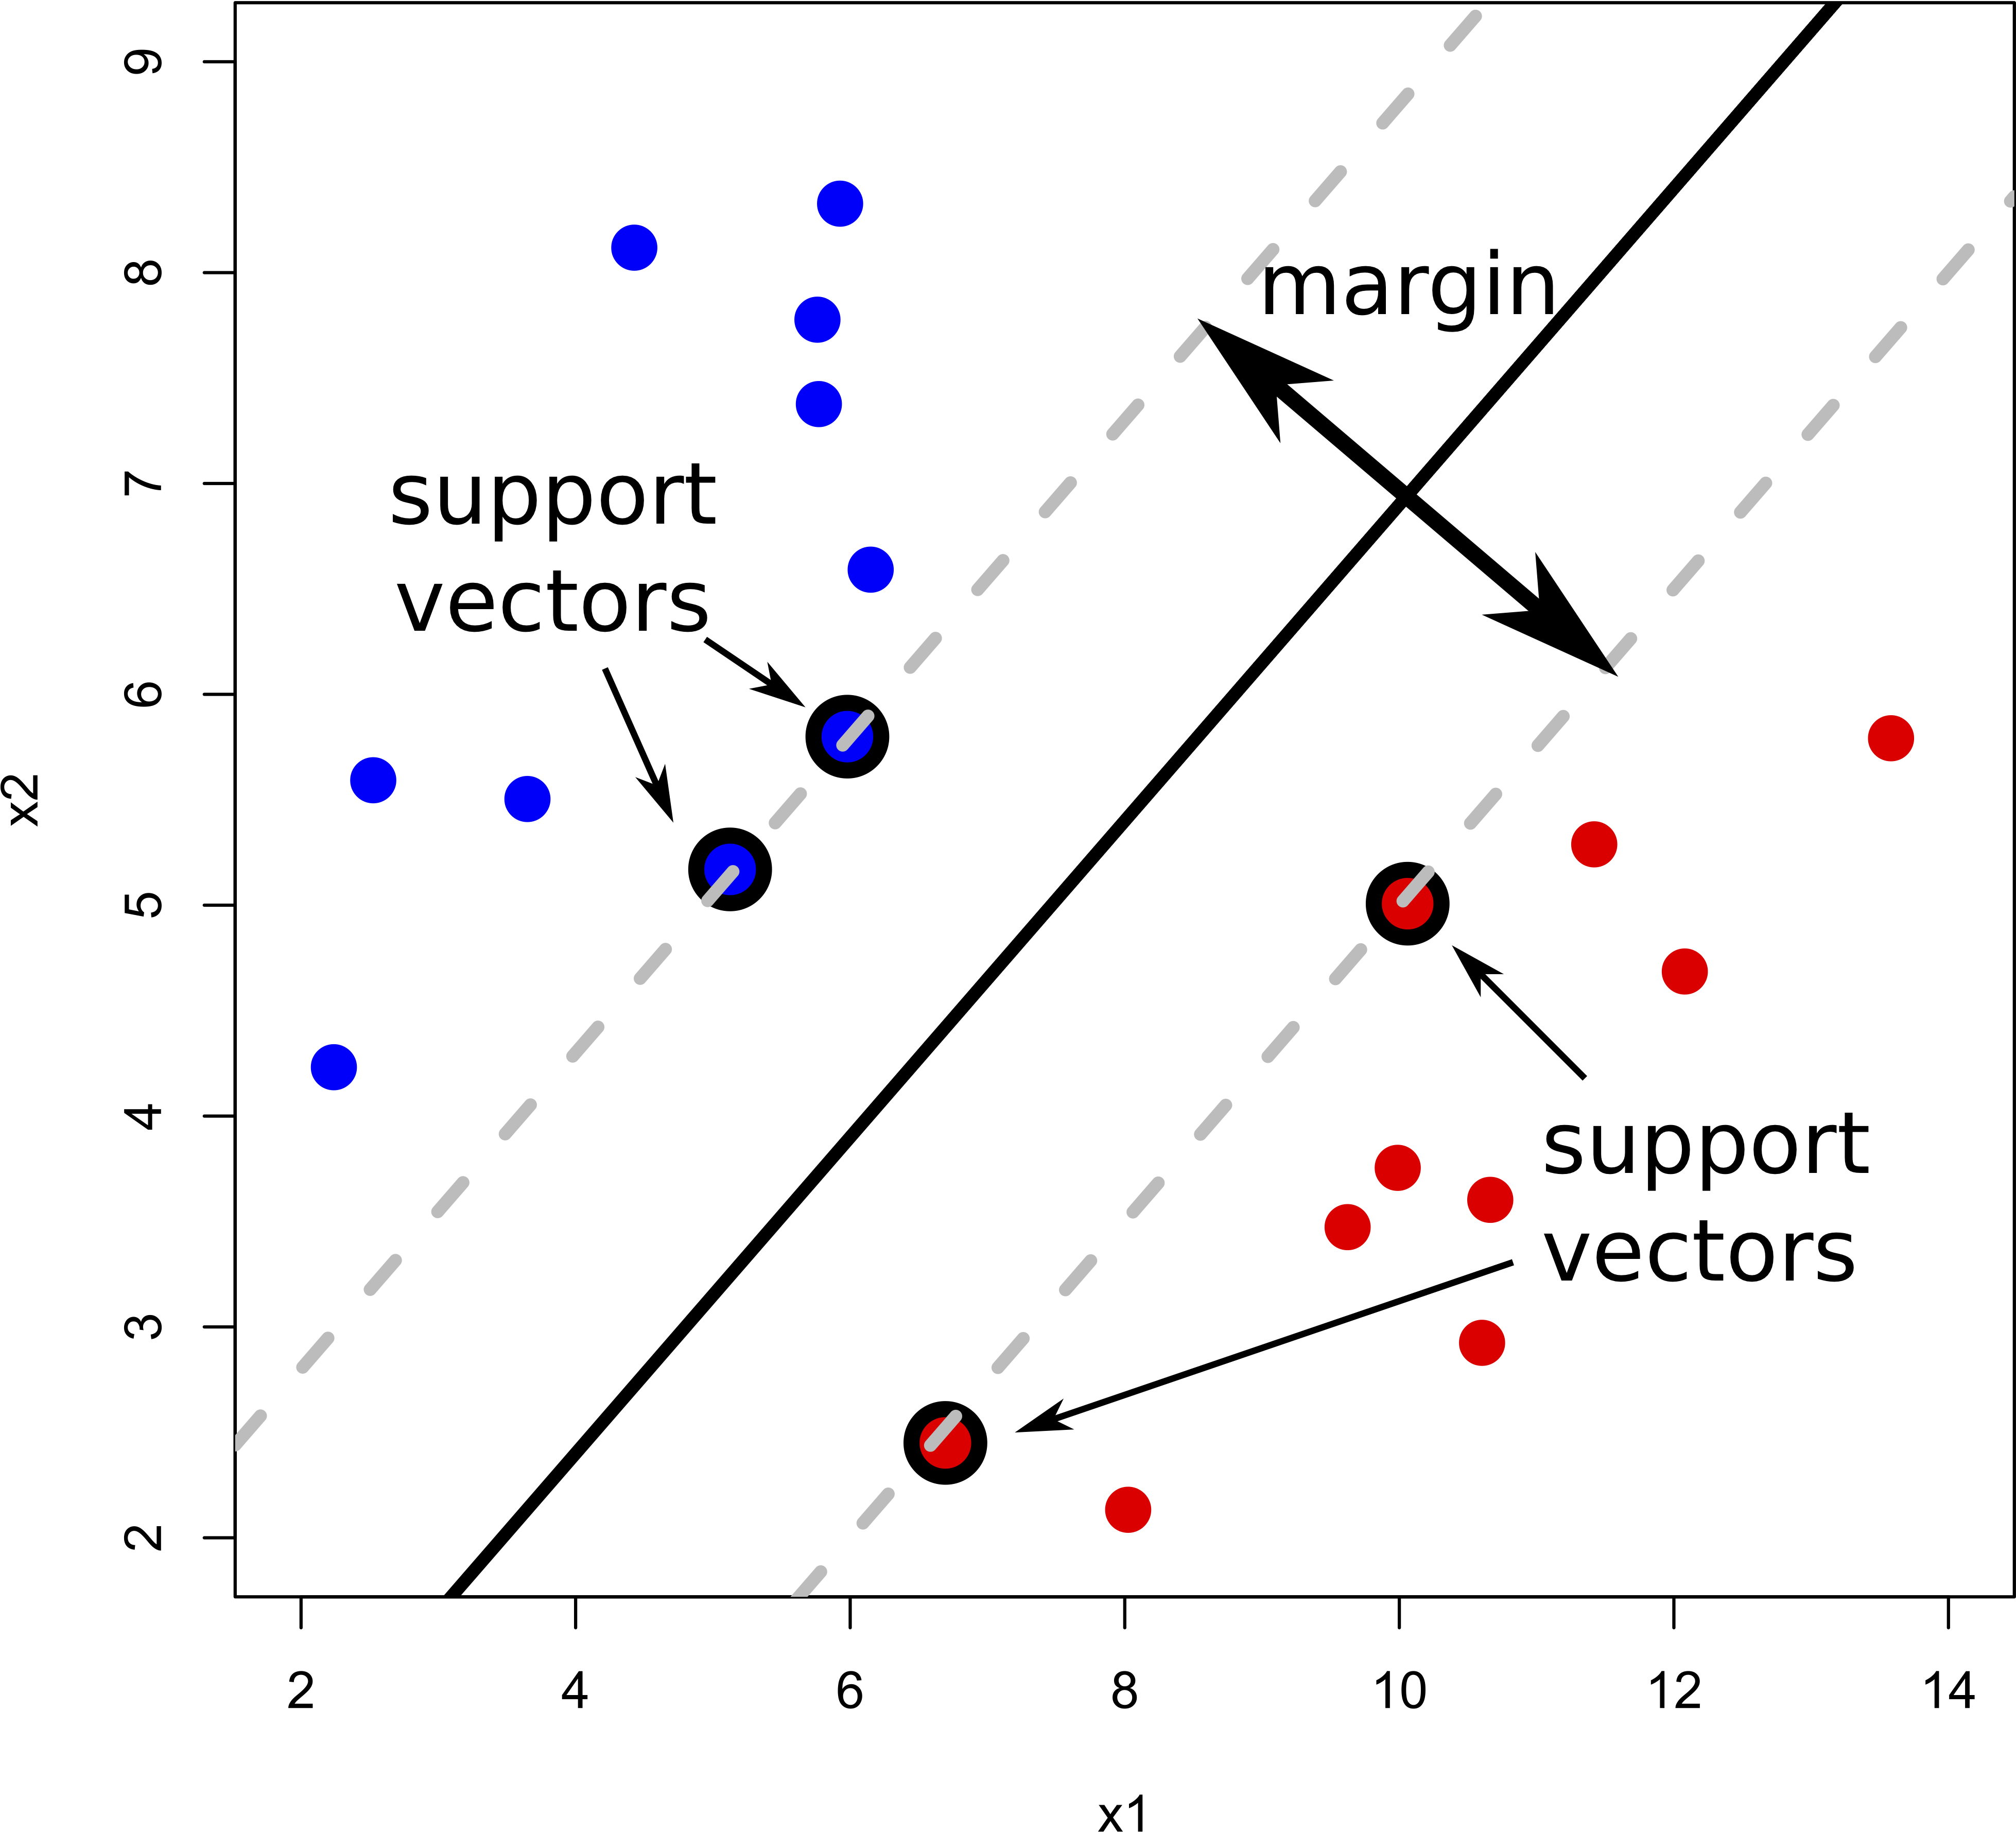
\includegraphics[width=0.65\textwidth]{04-svmsketch.png}
\end{center}
\end{frame}

%=============================================================================%
%=============================================================================%
\begin{frame}{Support vector classifiers}
\textbf{Rationale}: Use a \textit{soft} margin
\begin{center}
		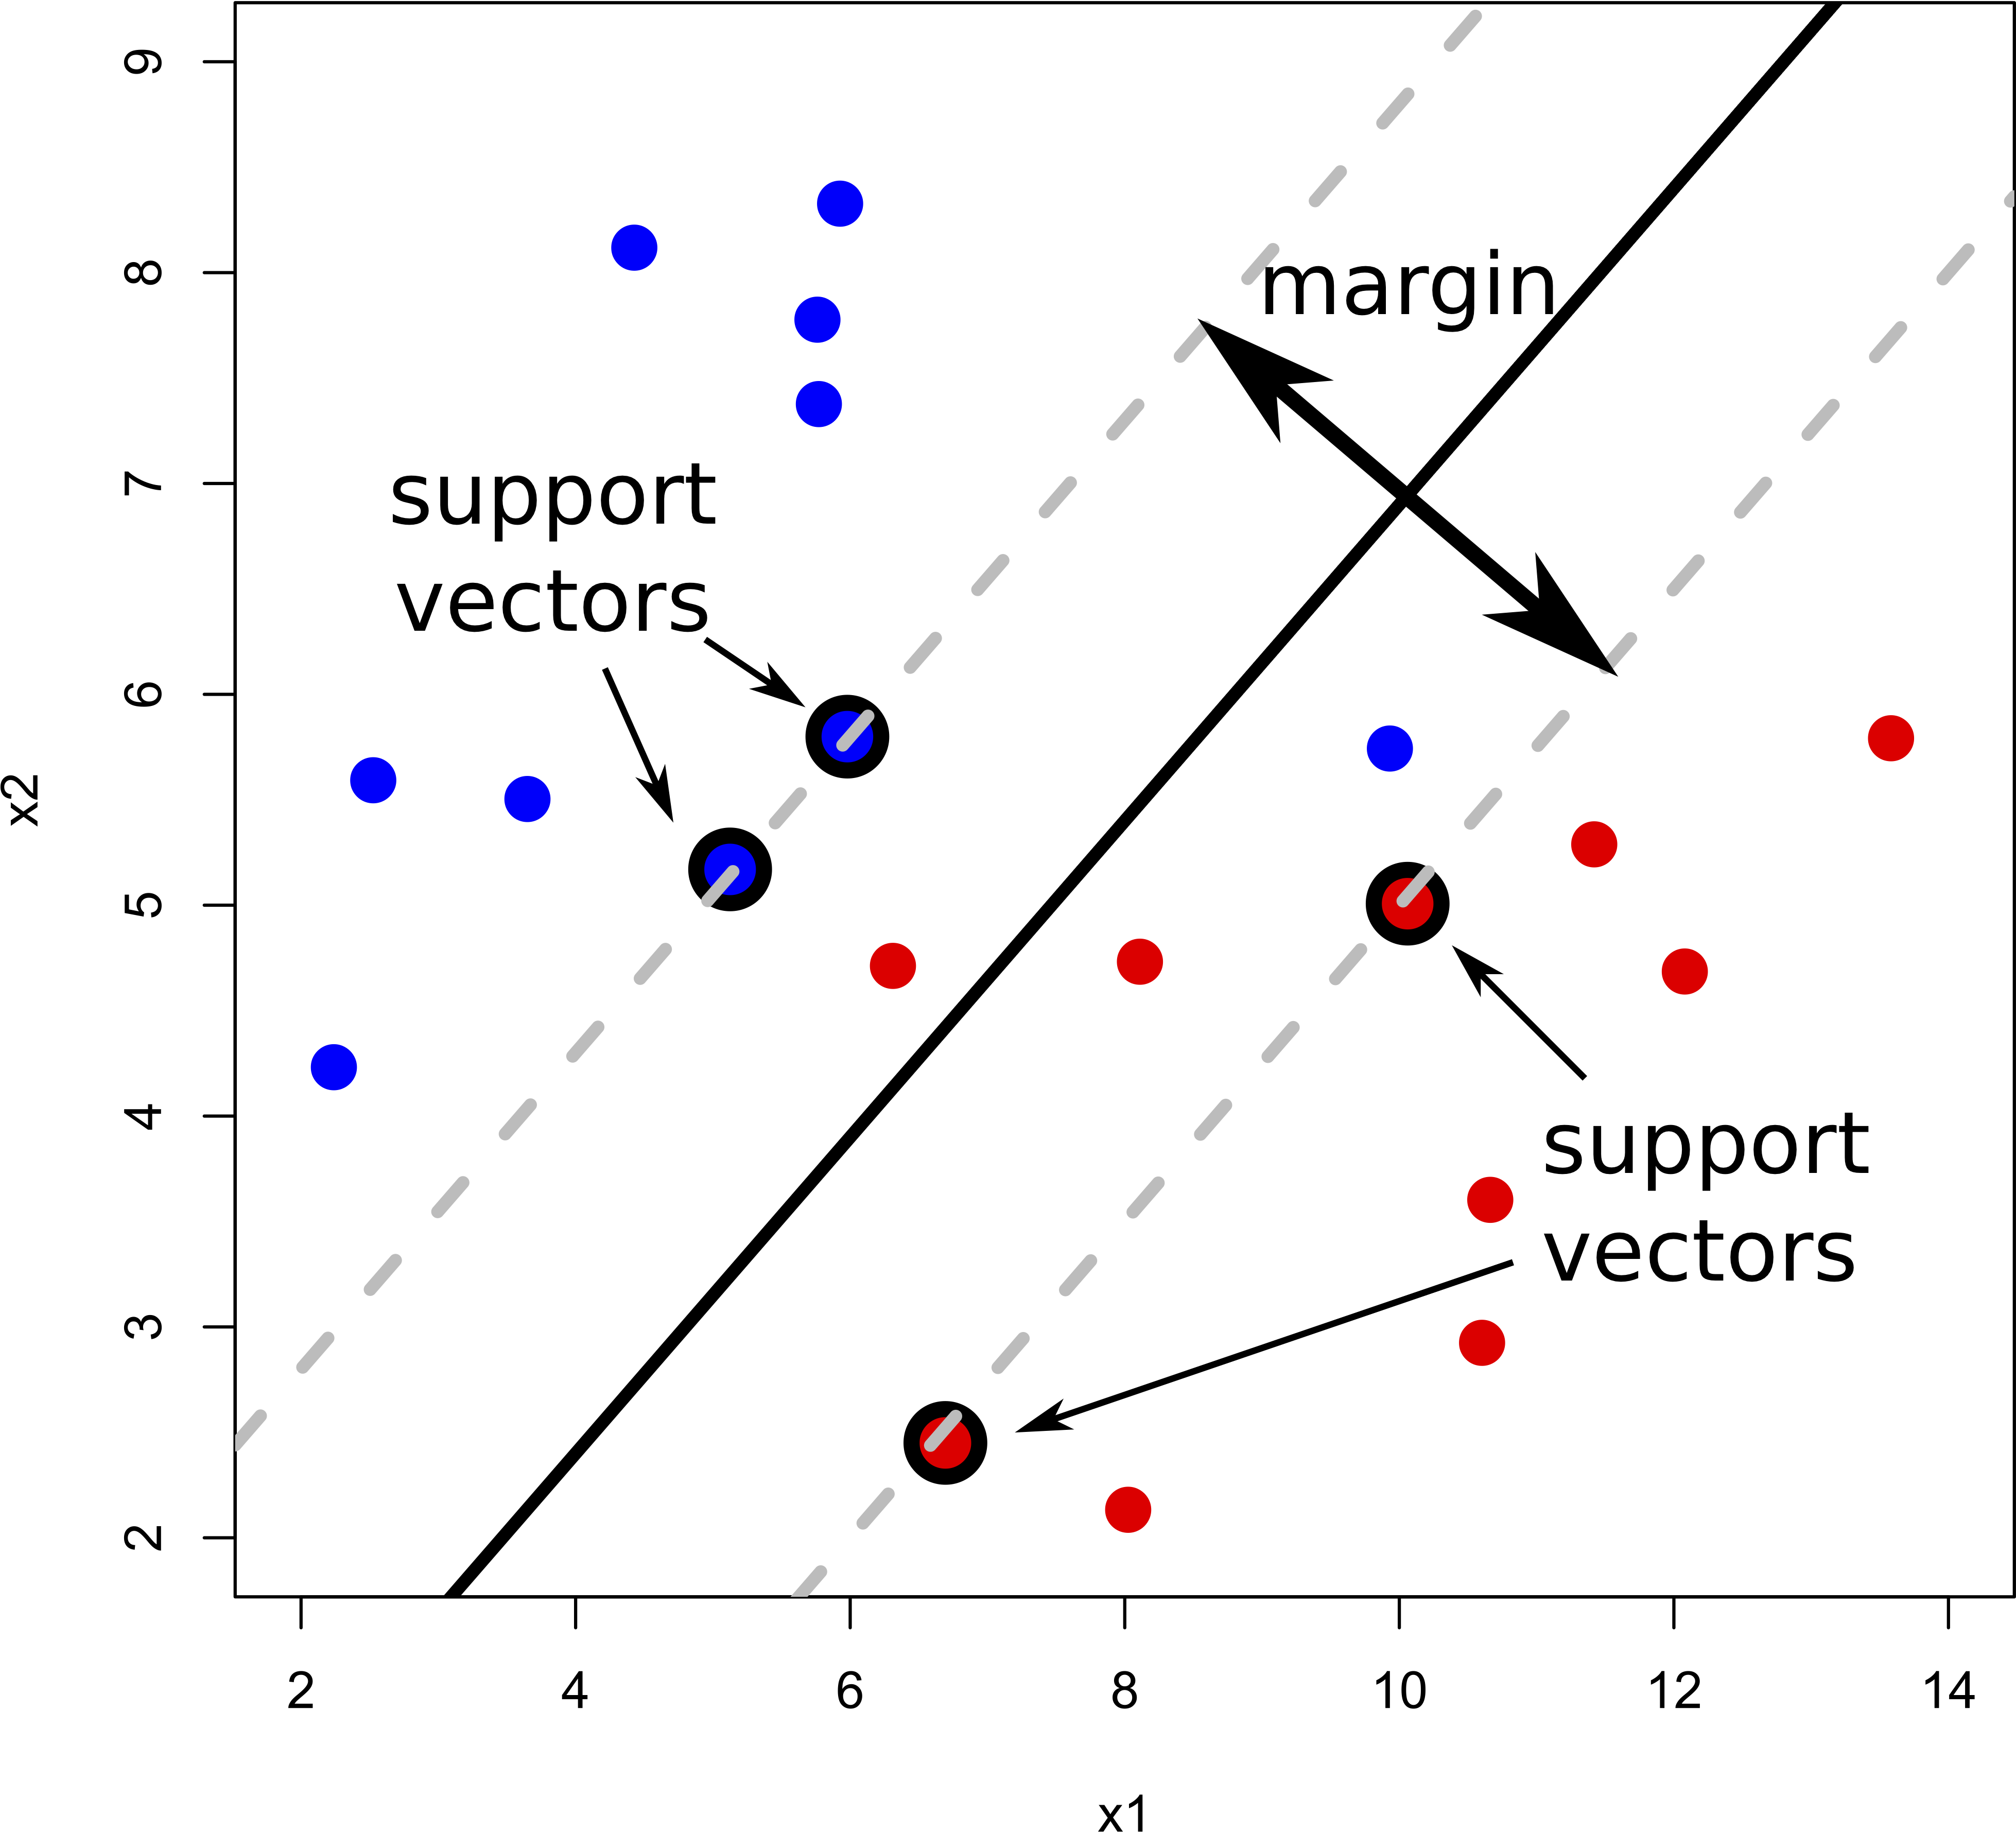
\includegraphics[width=0.65\textwidth]{04-svmsoft.png}
\end{center}
\end{frame}

%=============================================================================%
%=============================================================================%
\begin{frame}{Support vector machines}
Real-life data is complex and often we cannot find a separating hyperplane
\vfill
\begin{center}
		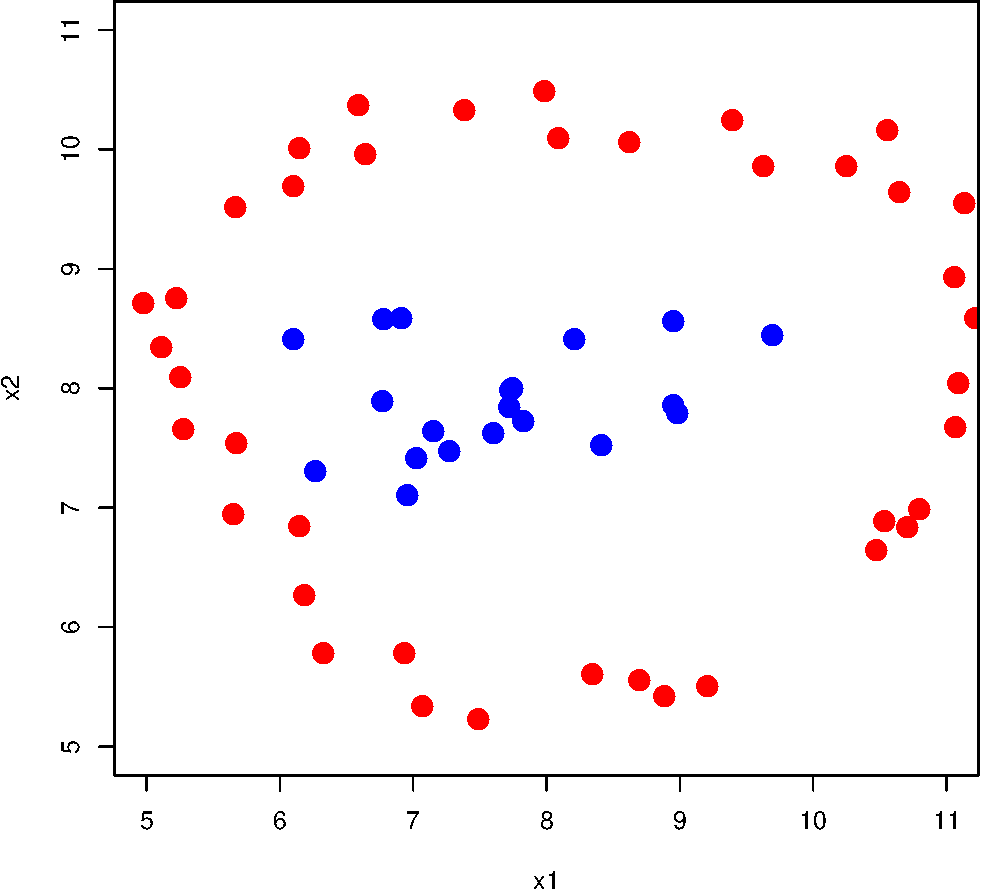
\includegraphics[width=0.6\textwidth]{svmNonLinear1.pdf}
\end{center}
\end{frame}

%=============================================================================%
%=============================================================================%
\begin{frame}{Support vector machines}
\textbf{Rationale}: Map data to a higher dimensional space where classes are linearly separable
\vfill
% \begin{itemize}
% 	\item $(x_1,\ x_2) \rightarrow (1,\ x_1,\ x_2,\ x_1x_2,\ x_1^2,\ x_2^2)$
% 	\item Hyperplane in \textit{new} space is a conic section in \textit{original} space 
% \end{itemize}
\begin{center}
		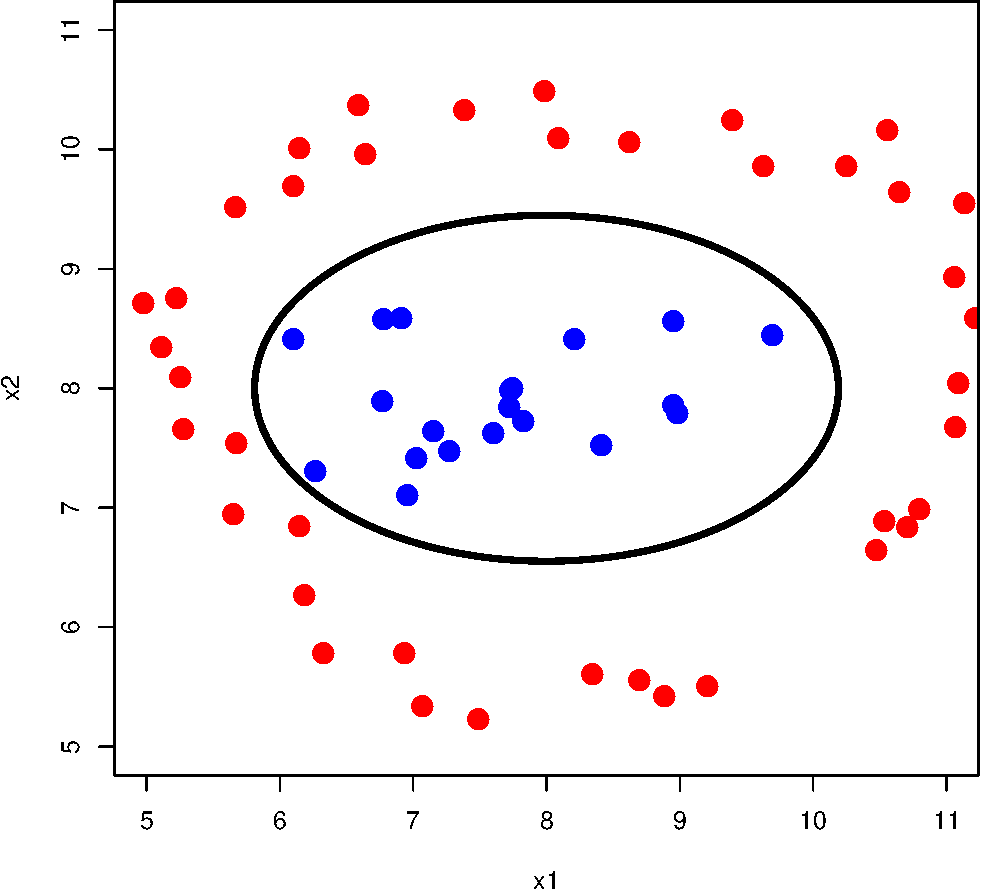
\includegraphics[width=0.6\textwidth]{svmNonLinear2.pdf}
\end{center}
\end{frame}

%=============================================================================%
%=============================================================================%
\begin{frame}{Support vector machines: 1D to 2D}
\begin{center}
		\visible<1->{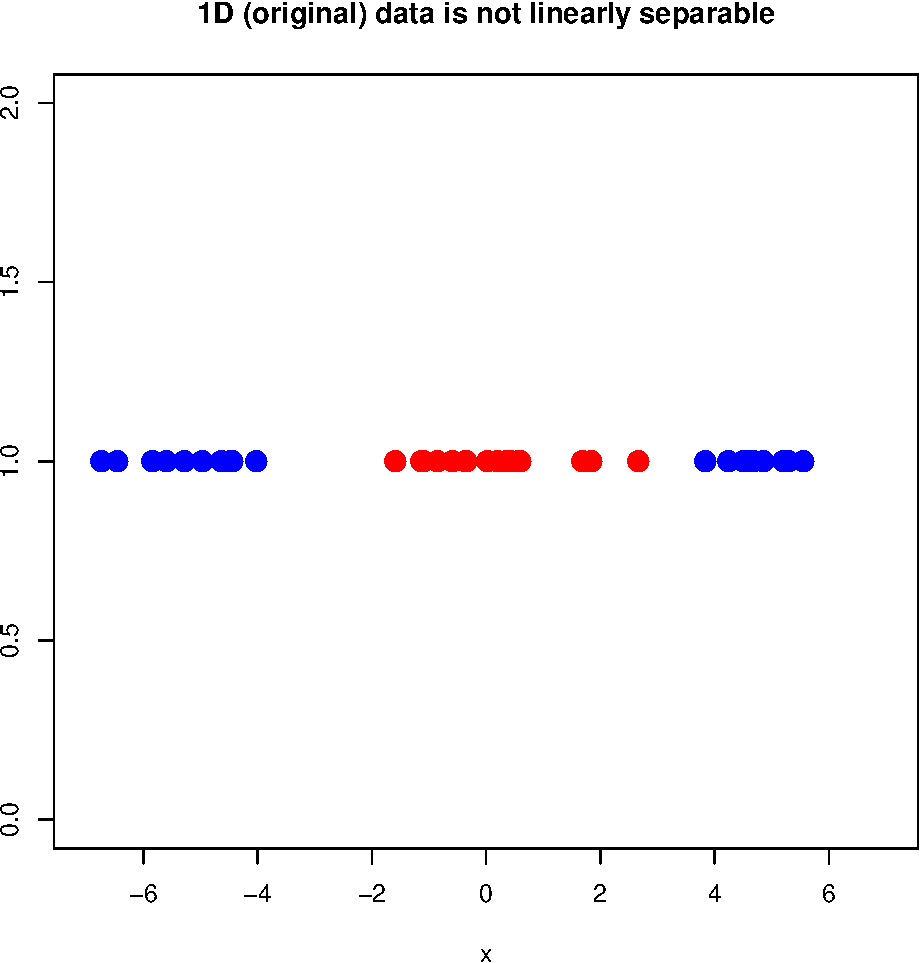
\includegraphics[width=0.47\textwidth]{svmSimple1.pdf}}
		\visible<2->{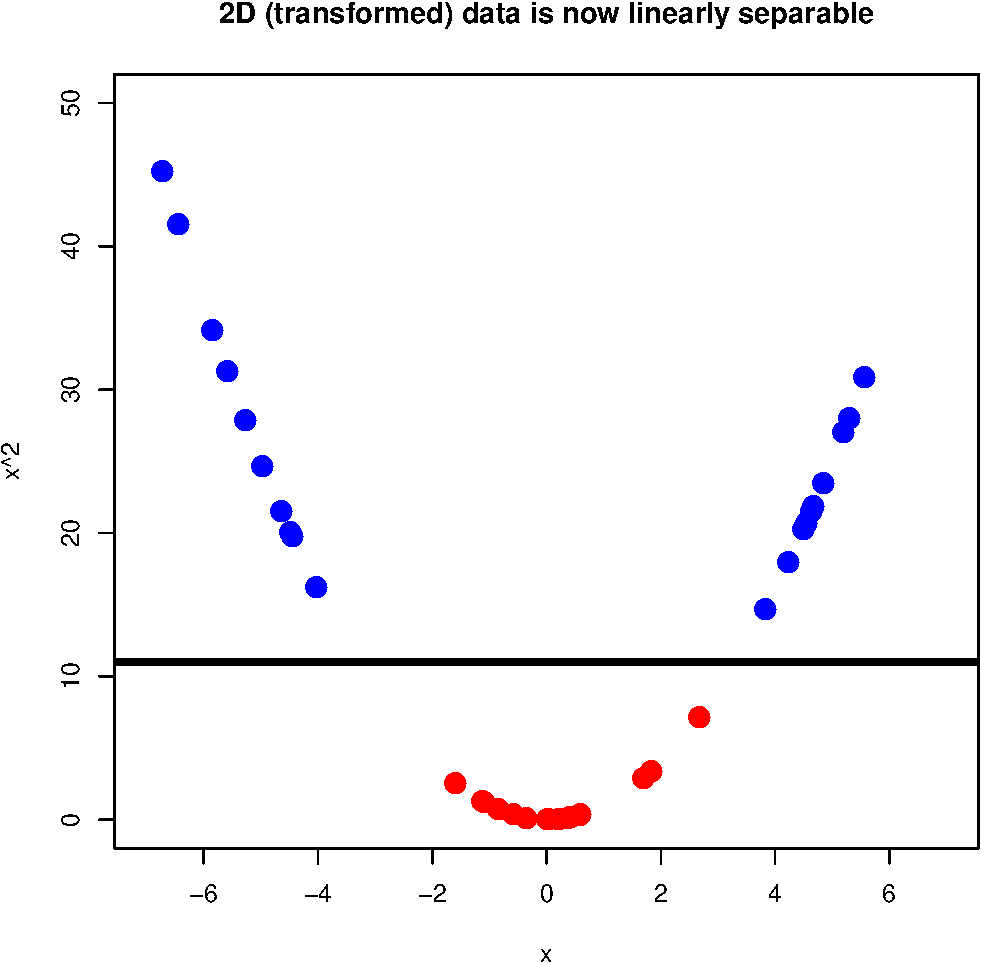
\includegraphics[width=0.50\textwidth]{svmSimple2.pdf}}
\end{center}
\end{frame}

%=============================================================================%
%=============================================================================%
\begin{frame}{Support vector machines - the kernel trick}
\begin{itemize}\addtolength{\itemsep}{0.25\baselineskip}
	\item So our solution is to blow up the dimensions?
	\item But what about the ``curse of dimensionality''?
	\item Very computationally expensive to work in high dimensions
\end{itemize}
\vfill
\visible<2->{\begin{block}{}
\begin{itemize}
	\item \textbf{Kernel trick} to the rescue! 
	\item Work in an \textit{implict} feature space
	\item Data is never explicitly computed in higher dimensions
	\item Think about kernels as generalised distance measures
\end{itemize}
\end{block}
\vfill
{\footnotesize \textbf{p.s} Kernel methods are mathematically intricate and beyond the scope of this introductory workshop}}
\end{frame}

%=============================================================================%
%=============================================================================%
\begin{frame}{Support vector machines}
\begin{enumerate}\addtolength{\itemsep}{2\baselineskip}
	\item Choose a kernel
	\item Run optimiser to find the maximum margin separating hyperplane
\end{enumerate}
\vfill
\visible<2->{
\begin{block}{}
SVMs are inherently binary classifiers. The most common ways to deal
with multi-class problems is by building several \textbf{one-versus-all} \textit{or} \textbf{one-versus-one}
classifiers. 
\end{block}}
\end{frame}

%=============================================================================%
%=============================================================================%
\begin{frame}{Support vector machines}
\begin{center}
		\includegraphics<1>[width=0.65\textwidth]{svmLinear.pdf}
		\includegraphics<2>[width=0.65\textwidth]{svmRBF.pdf}
\end{center}
\end{frame}

%=============================================================================%
%=============================================================================%
\begin{frame}{Support vector machines}
\begin{exampleblock}{Pros}
\begin{itemize}
	\item State-of-the-art predictive accuracy
	\item Low storage requirements (only support vectors to store)
	\item A vast array of kernels are available that are flexible enough to cater for any type of data
	\item Global optimum guaranteed
\end{itemize}
\end{exampleblock}
\vfill
\begin{alertblock}{Cons}
\begin{itemize}
	\item Model is hard to interpret
	\item Feature space cannot be visualised
\end{itemize}
\end{alertblock}
\end{frame}

%=============================================================================%
%=============================================================================%
\end{document}
%=============================================================================%
%=============================================================================%
% End of Document
%=============================================================================%
%=============================================================================%